\documentclass[11pt, a4]{article}
\newcommand{\lotteryset}{\mathcal{L}}
\newcommand{\outcomeset}{\mathcal{X}}
\usepackage{amssymb}
\usepackage{enumitem}
\usepackage{amsmath}
\usepackage{tfrupee}
\usepackage{pgfplots}
\usepackage{tikz}
\usepackage{enumitem}
\usepackage{multirow}
\usepackage{fancyhdr}
\usepackage{lastpage}
\usepackage[export]{adjustbox}
\usepackage{wrapfig}
\usepackage[english]{babel}
\usepackage{amsthm}
\usepackage{multirow}
\usepackage{wrapfig,lipsum,booktabs}
\usepackage{graphicx}
\usepackage{subcaption} 
\usepackage{float}
\usepackage{hyperref}

\topmargin -0.0in
% \textheight 11in
\oddsidemargin .5in
\evensidemargin 0.0in
\textwidth 5.5in

\begin{document}
	\pagestyle{fancy}
	\fancyhead{}\fancyfoot{}
	\fancyhead[L]{PA-1 Report}
	\fancyhead[C]{\thepage ~of \pageref{LastPage}}
	\fancyhead[R]{EE25S009}
	\author{Ritabrata Mandal\\ EE25S009}
	\title{EE5176: Computational Photography\\Programming Assignment-1: Basics of Imaging Report}
	\maketitle
	
	\medskip
%	\newpage
	\begin{enumerate}
		\item \textbf{Introduction}\\
		This assignment focuses on fundamental concepts in digital imaging, beginning with demosaicing and extending to noise removal. 
		All processed images generated during the assignment are available in the GitHub repository under the 
		\href{https://github.com/RitabrataMandal/EE5176/tree/master/Assignments/Assignment1/output}{\texttt{output}} folder.  
		
		\begin{enumerate}
			\item \textbf{Implementation}:\\
			The implementation has been carried out and tested in MATLAB R2025a. 
			A \texttt{main.m} script invokes four functions: \texttt{demos.m}, \texttt{white\_balance.m}, 
			\texttt{tone\_map.m}, and \texttt{denoising.m}. 
			The \texttt{demos.m} function performs image demosaicing for two given raw images, \texttt{RawImage1} and \texttt{kodim19}. 
			The functions \texttt{white\_balance.m} and \texttt{tone\_map.m} apply white balancing and tone mapping techniques, respectively, 
			on images such as \texttt{RawImage1}, \texttt{RawImage2} and \texttt{RawImage3}. Finally \texttt{denoising.m} apply bilateral filtering for denosing the same three images \texttt{RawImage1}, \texttt{RawImage2} and \texttt{RawImage3} 
			
			\item \textbf{Running the Code}:\\
			To execute the assignment, navigate to the \texttt{Assignment1} directory, run the \texttt{main.m} file, 
			and select options \texttt{1}, \texttt{2}, or \texttt{3} corresponding to the three tasks.
		\end{enumerate}
		
		\item \textbf{Demosaicing}\\
		Demosaicing is a process of interpolating the red, green and blue channels from
		the raw pixel image. Here we will try to fill in the missing pixel values from
		the sampled raw images through interpolation. \\
		 The CFA for \texttt{RawImage1.mat} is rggb whose mask is provided in the file
		\texttt{bayer1.mat}. In\texttt{ bayer1.mat} a value of 1 at a particular pixel means that only
		red value is sampled at that pixel. Similarly values of 2 and 3 mean that
		only green and blue values are sampled at those pixels. We use bilinear and
		bicubic interpolation for filling in the missing data. We interpolate only for
		those pixels whose values are missing in the grid. We use the MATLAB built-in
		function \texttt{griddata} for an efficient implementation.
		\begin{enumerate}
			\item Performing bilinear interpolation of the missing pixels in each color channel	R, G and B to reconstruct a full color image from \texttt{RawImage1} with the CFA provided in \texttt{bayer1.mat} and Figure \ref{fig:problem1_linear} shows the different color channel after interpolation. Figure \ref{fig:problem1_RGB_linear} shows the RGB reconstruction with linear interpolation
			\begin{figure}[H]
				\centering
				\resizebox{0.8\linewidth}{!}{
					\begin{tabular}{cc}
					\begin{subfigure}[h]{0.45\linewidth}
						\centering
						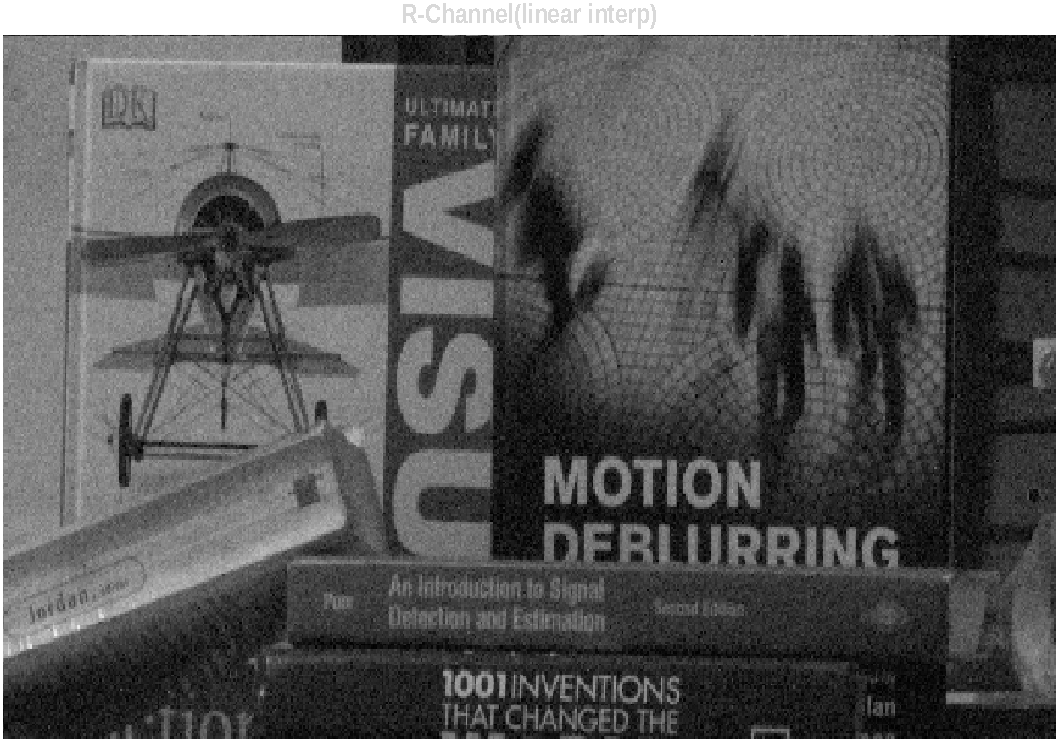
\includegraphics[width=\linewidth]{../output/1_R-channel_linear.pdf}
						\caption{R-Channel}
						\label{fig:problem1_R}
					\end{subfigure} &
					\begin{subfigure}[h]{0.45\linewidth}
						\centering
						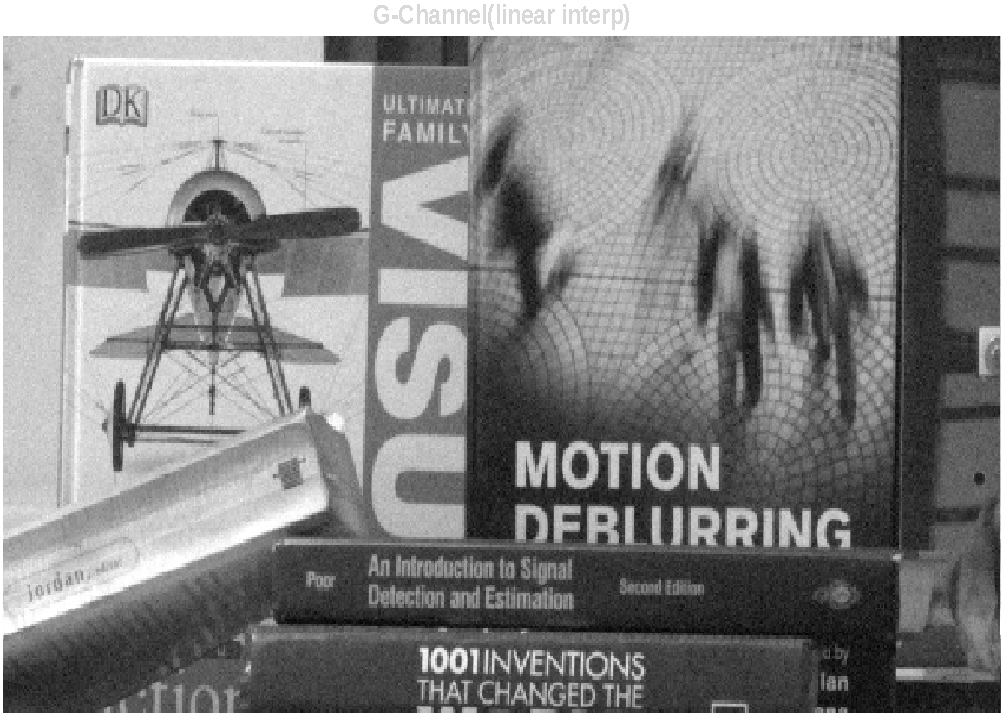
\includegraphics[width=\linewidth]{../output/1_G-channel_linear.pdf}
						\caption{G-Channel}
						\label{fig:problem1_G_linear}
					\end{subfigure}\\
					\begin{subfigure}[h]{0.45\linewidth}
						\centering
						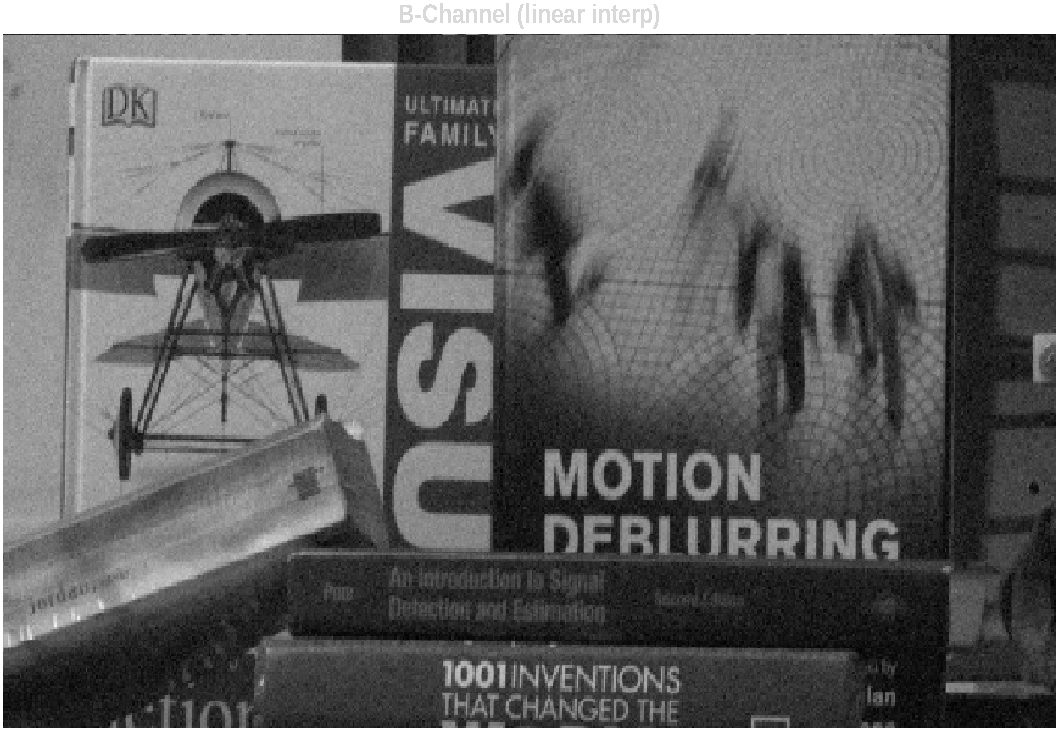
\includegraphics[width=\linewidth]{../output/1_B-channel_linear.pdf}
						\caption{B-Channel}
						\label{fig:problem1_B_linear}
					\end{subfigure} &
					\begin{subfigure}[h]{0.45\linewidth}
						\centering
						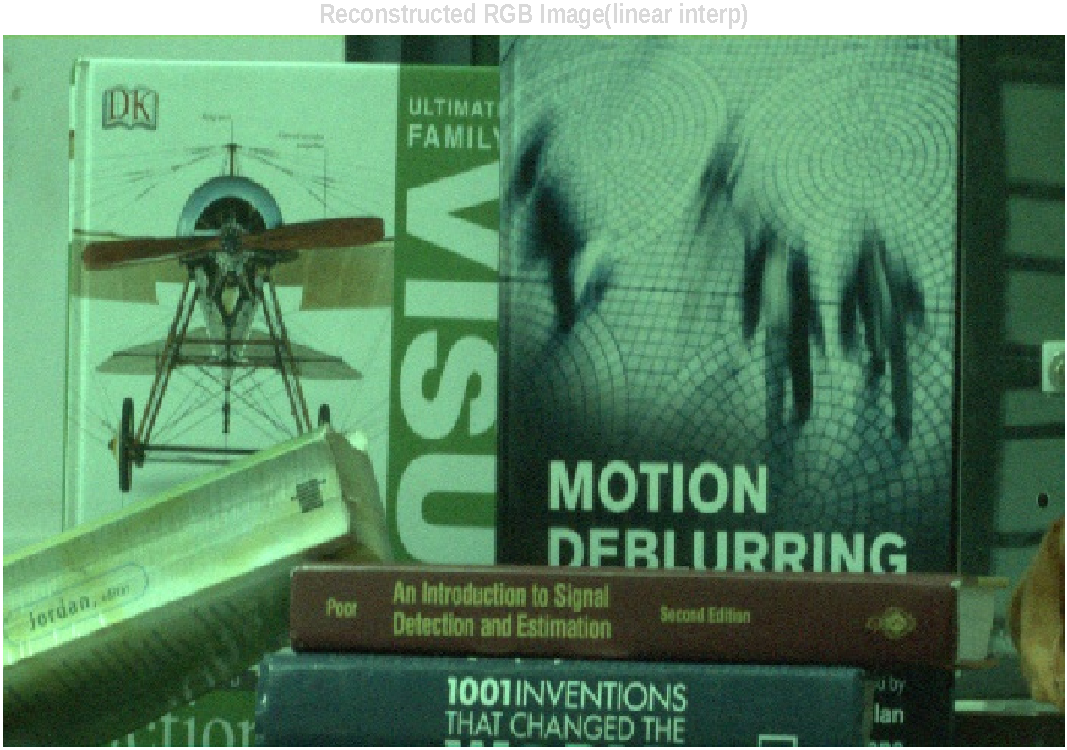
\includegraphics[width=\linewidth]{../output/1_RGB_linear.pdf}
						\caption{Reconstructed	RGB}
						\label{fig:problem1_RGB_linear}
					\end{subfigure}
				\end{tabular}
			}
%				\label{fig:problem1_linear}
				\caption{Reconstructed \texttt{RawImage1} with linear interpolation.}
				\label{fig:problem1_linear}
			\end{figure}
			
			\item  Performing bicubic interpolation of the missing pixels in each color channel	R, G and B to reconstruct a full color image from \texttt{RawImage1} with the CFA provided in \texttt{bayer1.mat} and Figure \ref{fig:problem1_cubic} shows the different color channel after interpolation. Figure~\ref{fig:problem1_RGB_cubic} shows the RGB reconstruction with cubic interpolation.\\
			\textbf{Comparision with Bilinear Interpolation:} When comparing the results of bicubic interpolation and bilinear interpolation, the images appear almost identical at first glance. However, on closer inspection by zooming in, bicubic interpolation produces sharper edges with less blurriness than bilinear interpolation. In general, unless we specifically look for these differences at higher magnification, it is difficult to distinguish between the two images.
			
			\begin{figure}[H]
				\centering
				\resizebox{0.8\linewidth}{!}{ 
					\begin{tabular}{cc}
						\begin{subfigure}[h]{0.45\linewidth}
							\centering
							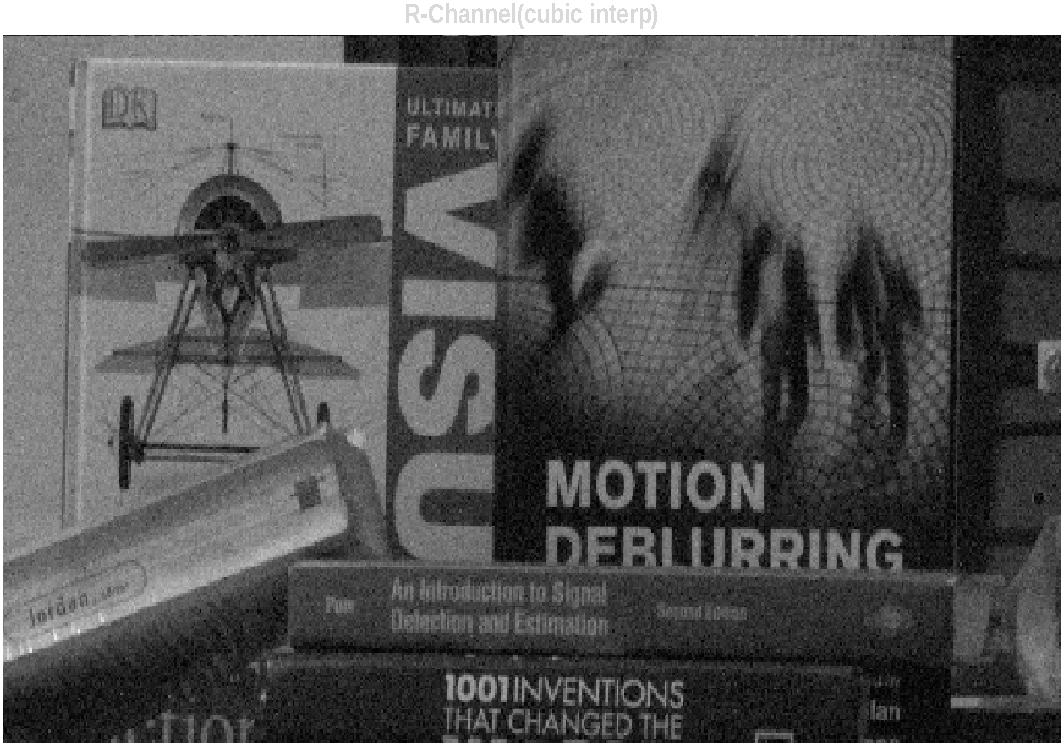
\includegraphics[width=\linewidth]{../output/1_R-channel_cubic.pdf}
							\caption{R-Channel}
							\label{fig:problem1_R_cubic}
						\end{subfigure} &
						\begin{subfigure}[h]{0.45\linewidth}
							\centering
							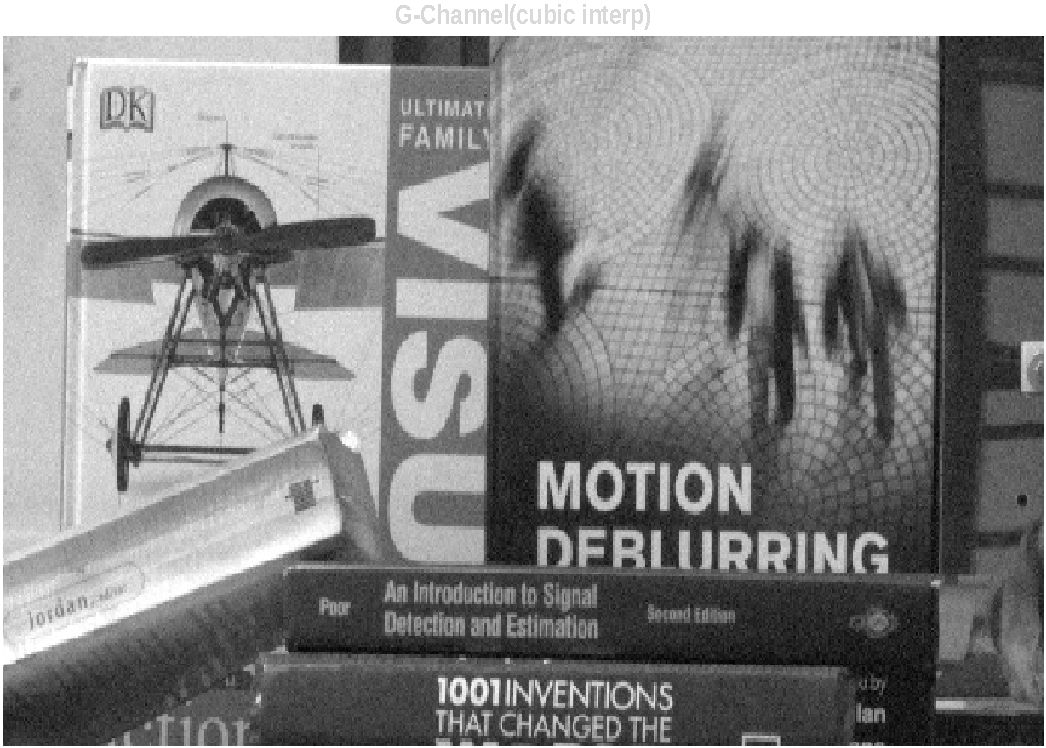
\includegraphics[width=\linewidth]{../output/1_G-channel_cubic.pdf}
							\caption{G-Channel}
							\label{fig:problem1_G_cubic}
						\end{subfigure} \\
						\begin{subfigure}[h]{0.45\linewidth}
							\centering
							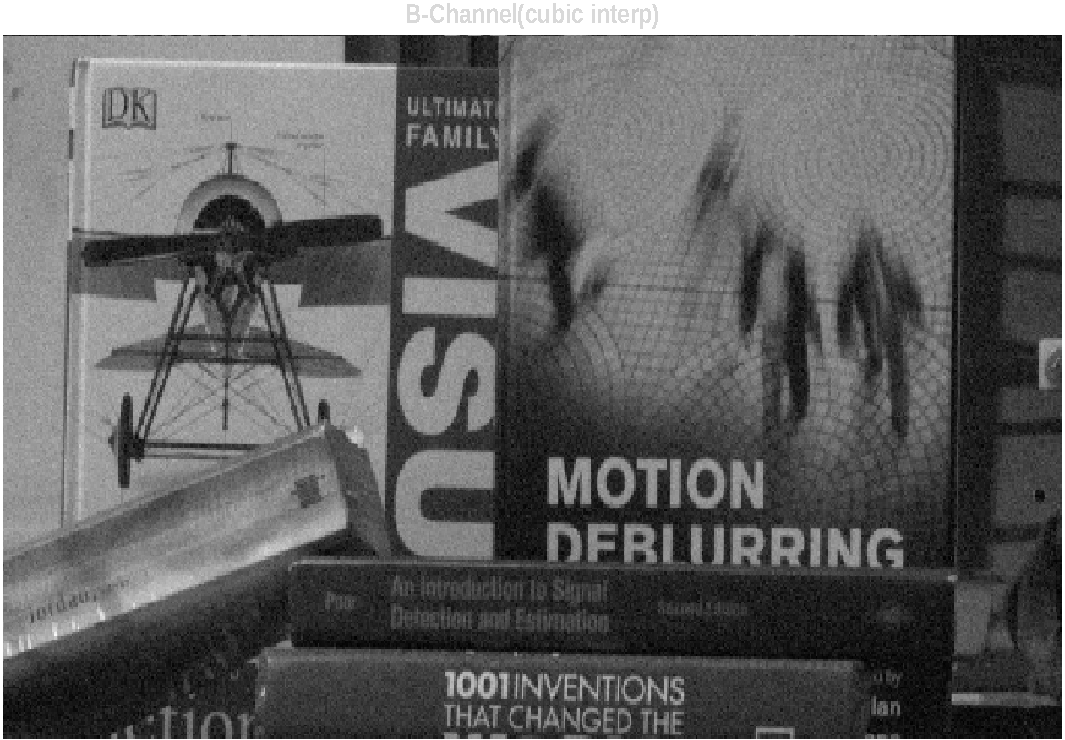
\includegraphics[width=\linewidth]{../output/1_B-channel_cubic.pdf}
							\caption{B-Channel}
							\label{fig:problem1_B_cubic}
						\end{subfigure} &
						\begin{subfigure}[h]{0.45\linewidth}
							\centering
							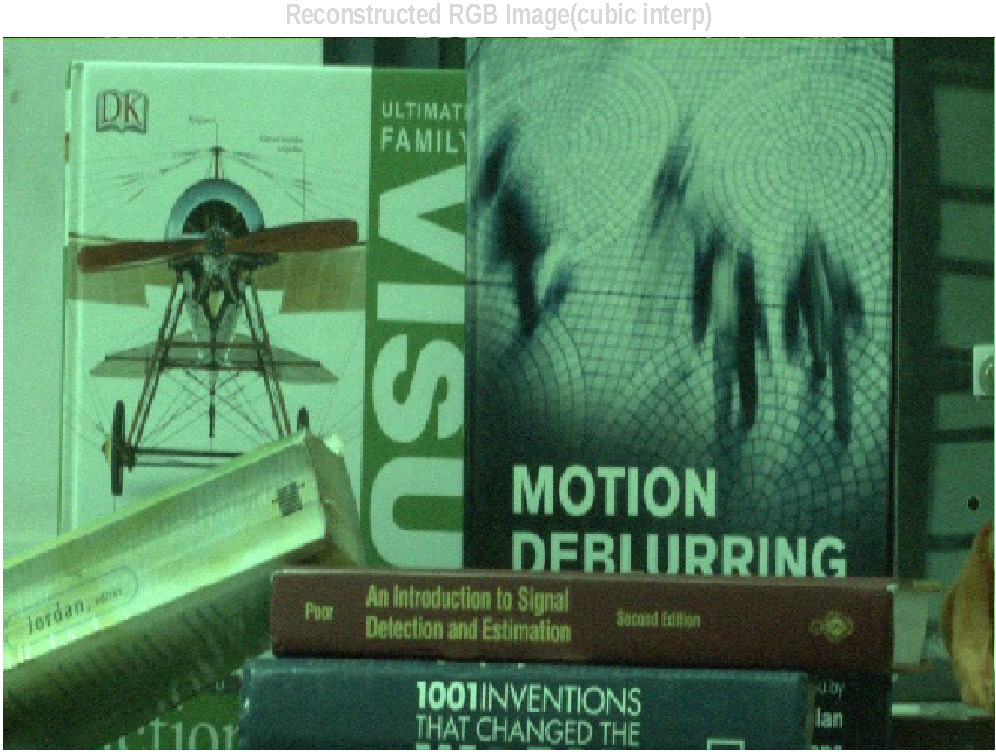
\includegraphics[width=\linewidth]{../output/1_RGB_cubic.pdf}
							\caption{Reconstructed RGB}
							\label{fig:problem1_RGB_cubic}
						\end{subfigure}
					\end{tabular}
				}
				\caption{Reconstructed \texttt{RawImage1} with cubic interpolation.}
				\label{fig:problem1_cubic}
			\end{figure}
			
			\item As shown in Figure~\ref{fig:problem1_inbuild}, the \texttt{RawImage1} was demosaiced using the rggb pattern with MATLAB’s built-in function \texttt{demosaic}.\\
			\textbf{Comparison with Interpolation Methods:}\\
			The three interpolation methods produce images that look quite similar, with differences only noticeable upon zooming in. In such cases, the \texttt{demosaic} function retains edge information more effectively, giving sharper results. Since \texttt{RawImage1} contains little high-frequency content, even bilinear interpolation performs well, though tone-mapped outputs from \texttt{demosaic} show a purple hue compared to the more neutral colors of bicubic interpolation.  
			
			
			\begin{figure}[H]
				\centering
				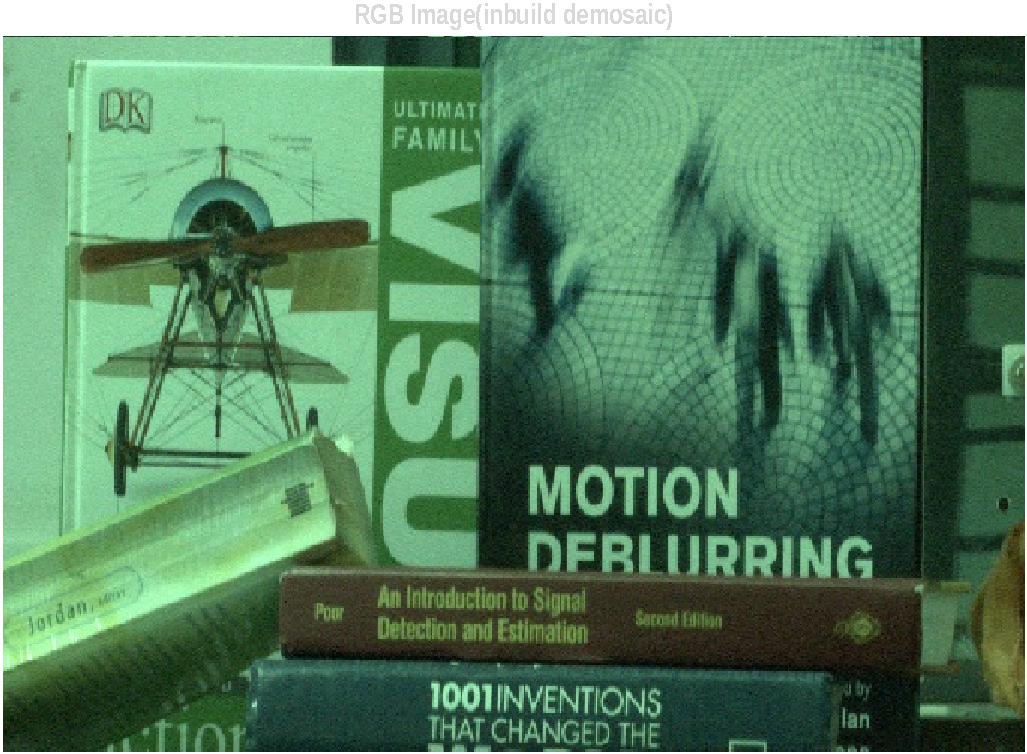
\includegraphics[width=0.5\linewidth]{../output/1_RGB_inbuild.pdf}
				\caption{Reconstructed \texttt{RawImage1} with \texttt{demosaic} function}
				\label{fig:problem1_inbuild}
			\end{figure}
			\item \textbf{Assumptions in Interpolation of Missing Pixel Values:}  
			\begin{enumerate}
				\item \textbf{Local Smoothness:} The image intensity is assumed to vary smoothly in a local neighborhood.  
				\item \textbf{Correlation of Neighboring Pixels:} Adjacent pixels are assumed to have similar values, especially within homogeneous regions.  
				\item \textbf{Limited High-Frequency Content:} The image is assumed to have relatively low noise and not contain abrupt intensity changes at small scales.  
				\item \textbf{Edge Continuity:} Edges are assumed to be continuous, allowing interpolation methods to preserve structure without introducing artifacts.  
			\end{enumerate}
			
			\textbf{Consequences When Assumptions Do Not Hold:}  
			\begin{enumerate}
				\item \textbf{Loss of Detail:} If the image has high-frequency textures, interpolation may blur fine details.  
				\item \textbf{Artifacts:} Discontinuities in intensity (e.g., at edges) may cause artifacts such as color fringing or checkerboard patterns.  
				\item \textbf{Distortion of Structures:} Interpolated pixels may not follow the true underlying structure, leading to edge distortion.  
				\item \textbf{Noise Amplification:} In the presence of noise, interpolation may reinforce or spread the noise instead of reconstructing the true signal.  
			\end{enumerate}
			
			\item Performing bicubic interpolation on \texttt{kodim19.mat} which has been sampled
			with the CFA pattern ‘RGGB’ to reconstruct a full color image shown in Figure~\ref{fig:problem1_part2}.
			\begin{figure}[H]
				\centering
				\resizebox{.8\linewidth}{!}{
					\begin{tabular}{cc}
					\begin{subfigure}[h]{0.45\linewidth}
						\centering
						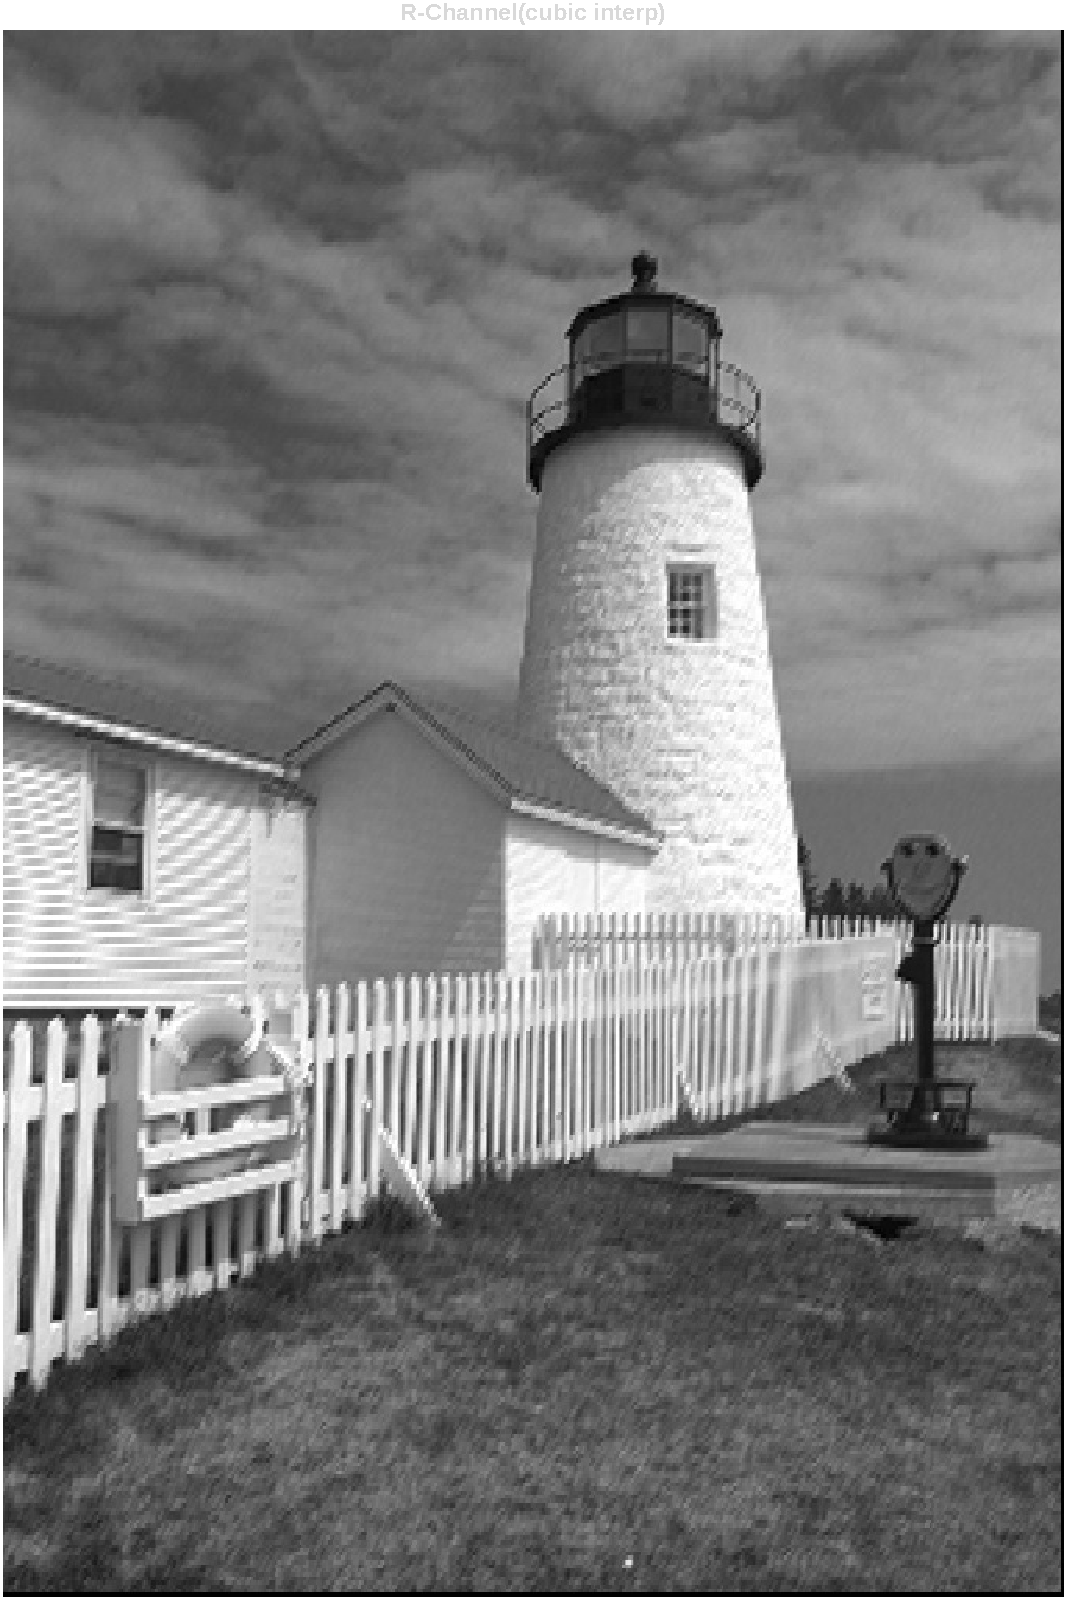
\includegraphics[width=\linewidth]{../output/2_R-channel_cubic.pdf}
						\caption{R-Channel}
						\label{fig:problem1_part2_R_cubic}
					\end{subfigure} &
					\begin{subfigure}[h]{0.45\linewidth}
						\centering
						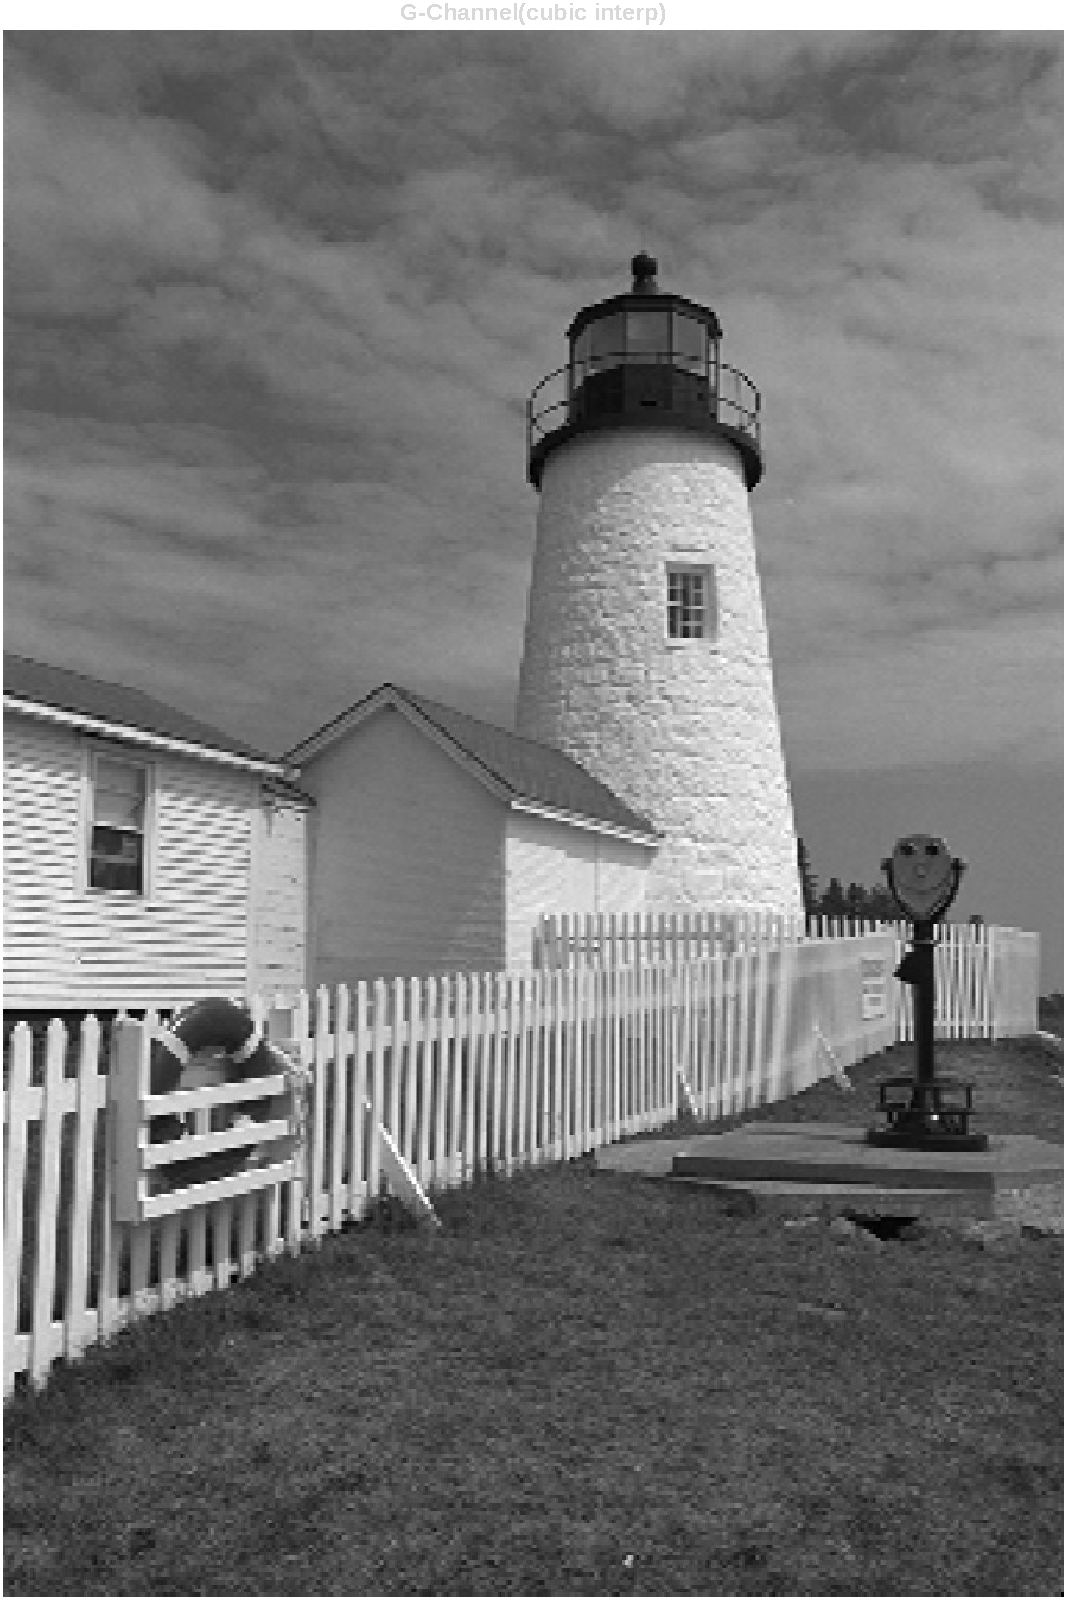
\includegraphics[width=\linewidth]{../output/2_G-channel_cubic.pdf}
						\caption{G-Channel}
						\label{fig:problem_part21_G_cubic}
					\end{subfigure}\\
					\begin{subfigure}[h]{0.45\linewidth}
						\centering
						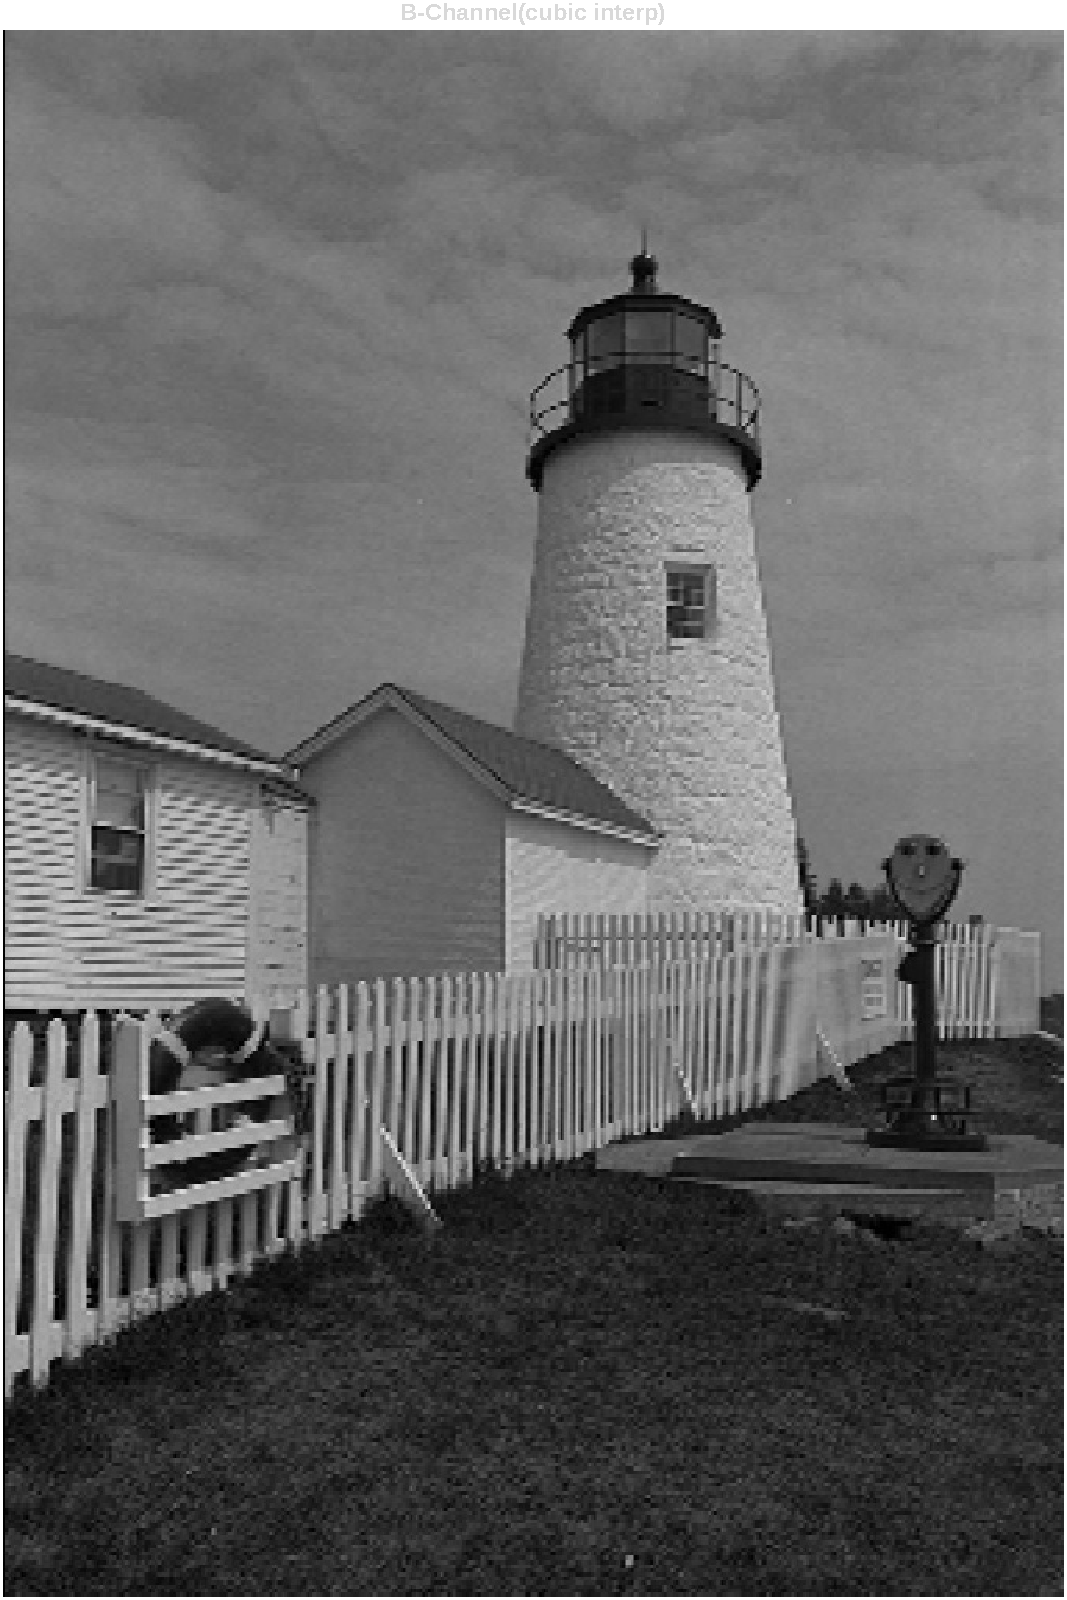
\includegraphics[width=\linewidth]{../output/2_B-channel_cubic.pdf}
						\caption{B-Channel}
						\label{fig:problem1_part2_B_cubic}
					\end{subfigure} &
					\begin{subfigure}[h]{0.45\linewidth}
						\centering
						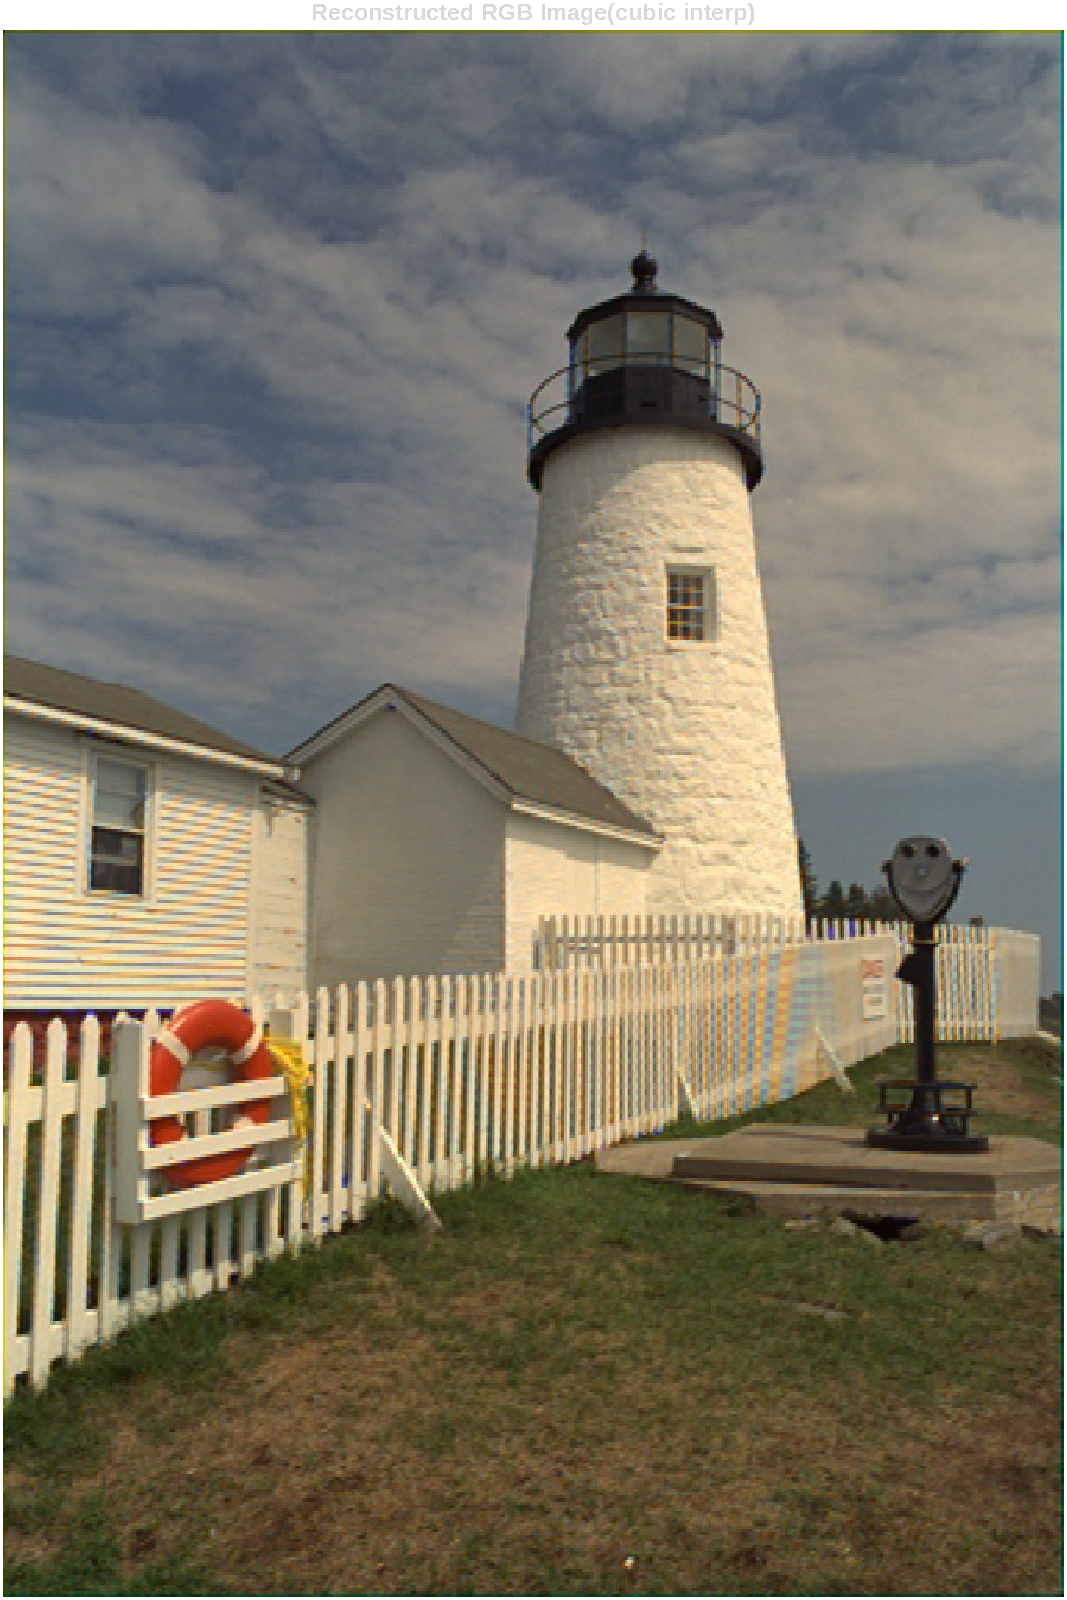
\includegraphics[width=\linewidth]{../output/2_RGB_cubic.pdf}
						\caption{Reconstructed RGB}
						\label{fig:problem1_part2_cubic}
					\end{subfigure}
					\end{tabular}
				}
				\caption{Reconstructed \texttt{kodim19.mat} with cubic interpolation.}
				\label{fig:problem1_part2}
			\end{figure}
			\item Now taking the Figure \ref{fig:problem1_part2_cubic} converting to YCrCb and applying the median filter to the chrominance channels and then converting back it to RGB channel. We get Figure \ref{fig:problem_part2}
			\begin{figure}[H]
				\centering
				\resizebox{0.8\linewidth}{!}{
					\begin{tabular}{cc}
						\begin{subfigure}[h]{0.45\linewidth}
							\centering
							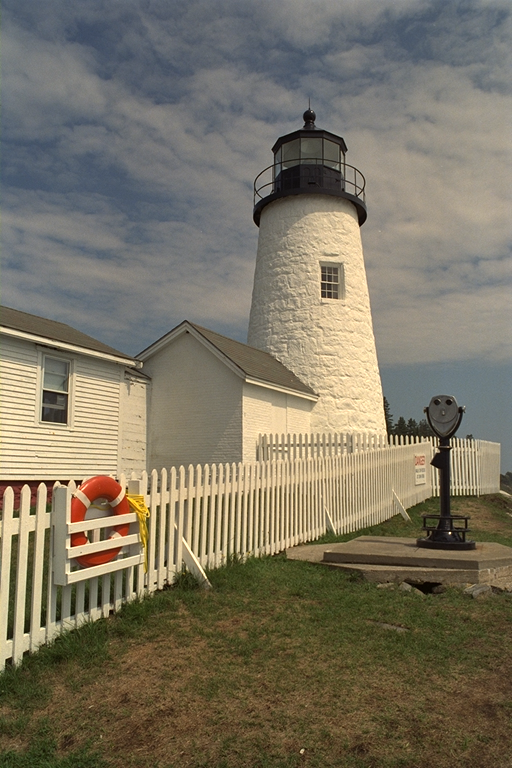
\includegraphics[width=\linewidth]{../kodim19.png}
							\caption{\texttt{kodim19} original}
							\label{fig:kodim19_original}
						\end{subfigure} &
						\begin{subfigure}[h]{0.455\linewidth}
							\centering
							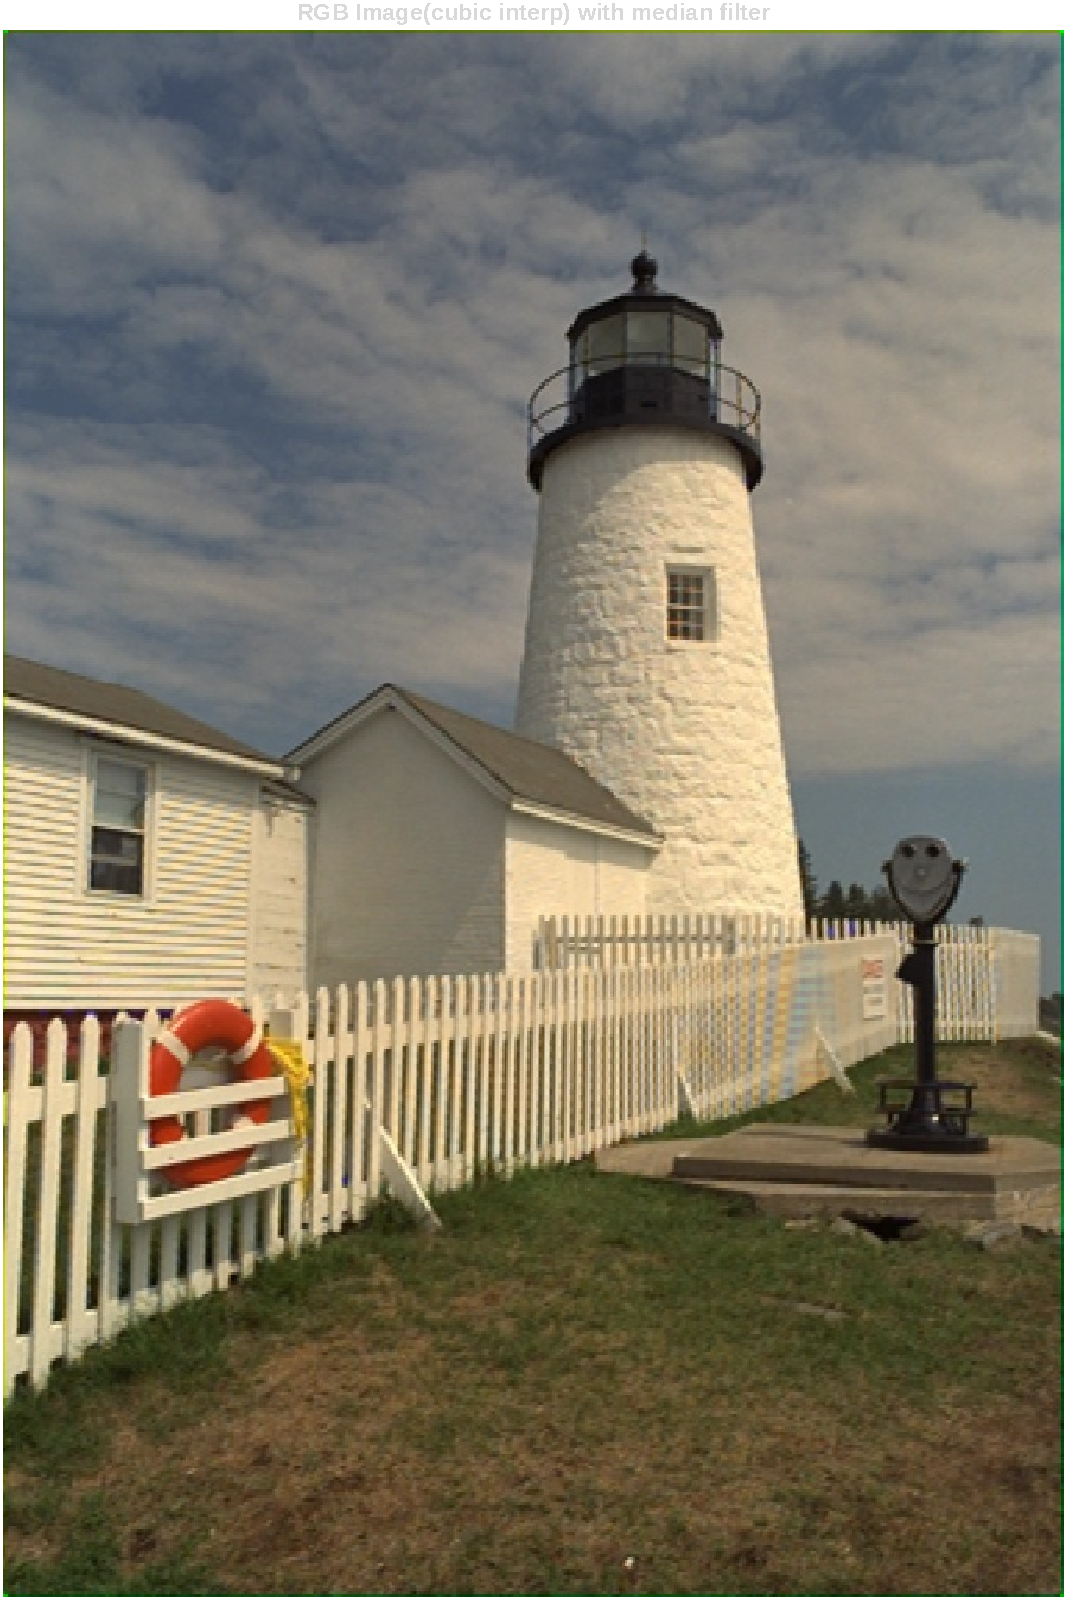
\includegraphics[width=\linewidth]{../output/2_RGB_cubic_median.pdf}
							\caption{Median after reconstruction}
							\label{fig:problem_part2}
						\end{subfigure}
					\end{tabular}
					}
					\caption{\texttt{kodim19.mat} original and median filter with cubic interpolation.}
					\label{fig:problem1_original}
				\end{figure}
			\item In the Figure \ref{fig:problem1_part2_cubic} (i.e. cubic interpolated rgb) we can see  moire pattern where as in Figure \ref{fig:problem_part2}(i.e. after applying median filter in chrominance channel) there is less moire pattern present in the image. Figure \ref{fig:kodim19_original} shows the original \texttt{kodim19.png}
		\end{enumerate}
		\item \textbf{White Balancing and Tone Mapping}\\
		In this section, we perform white balancing and tone mapping on \texttt{RawImage1}, \texttt{RawImage2}, and \texttt{RawImage3}. The built-in \texttt{demosaic} function is used to reconstruct full-color images from the raw sensor data. White balancing is carried out using three different approaches:  
		\begin{itemize}
			\item Assuming the average color of the scene is gray (gray-world assumption). 
			\item Assuming the brightest pixel represents a specular highlight and should therefore be white. 
			\item Assuming that a specific region of the scene is neutral. 
		\end{itemize}
		
		Once the images are white-balanced, tone mapping is applied using two methods:  
		\begin{itemize}
			\item Histogram equalization  
			\item Gamma correction with $\gamma \in \{0.5, 0.7, 0.9\}$  
		\end{itemize}
		
		The white balancing results are summarized as follows:  
		\begin{enumerate}
			\item \textbf{Gray-world assumption:} The mean value of each channel is computed, and scaling factors are applied to shift the average color toward gray. Figure \ref{fig:RawImage1_WB_2} shows the result for \texttt{RawImage1}, while Figure \ref{fig:RawImage2_WB_2} and Figure \ref{fig:RawImage3_WB_2} present the corresponding results for \texttt{RawImage2} and \texttt{RawImage3}.
			\item \textbf{Specular highlight assumption:} The brightest pixel is assumed to be white. Using the specified pixel coordinates $(830, 814)$ for \texttt{RawImage1}, $(1165, 280)$ for \texttt{RawImage2}, and $(175, 675)$ for \texttt{RawImage3}, the results are shown in Figure \ref{fig:RawImage1_WB_3}, Figure \ref{fig:RawImage2_WB_3}, and Figure \ref{fig:RawImage3_WB_3}.
			\item \textbf{Neutral region assumption:} A selected region is assumed neutral. The chosen pixel coordinates are $(2000, 435)$ for \texttt{RawImage1}, $(445, 715)$ for \texttt{RawImage2}, and $(1550, 565)$ for \texttt{RawImage3}. The results are presented in Figure \ref{fig:RawImage1_WB_4}, Figure \ref{fig:RawImage2_WB_4}, and Figure \ref{fig:RawImage3_WB_4}.
			\item \textbf{Tone mapping:} After white balancing, tone mapping is performed on all three images. The results are shown in Figure \ref{fig:RawImage1_tone}, Figure \ref{fig:RawImage2_tone}, and Figure \ref{fig:RawImage3_tone}.
		\end{enumerate}
			\begin{figure}[h]
				\centering
				\resizebox{0.8\linewidth}{!}{
					\begin{tabular}{cc}
						\begin{subfigure}[h]{0.45\linewidth}
							\centering
							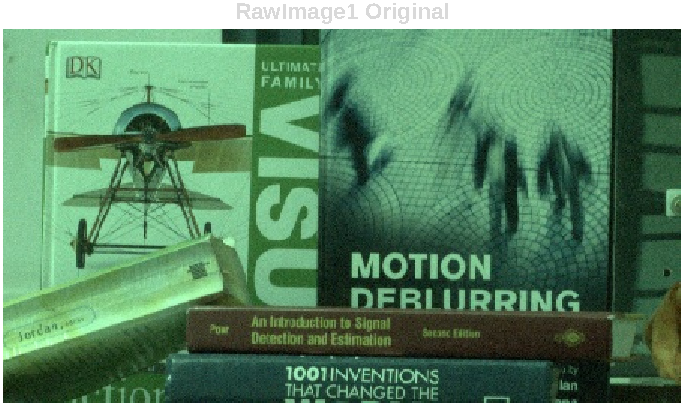
\includegraphics[width=\linewidth]{../output/RawImage1_WB_1.pdf}
							\caption{RawImage1 Original}
							\label{fig:RawImage1_WB_1}
						\end{subfigure} &
						\begin{subfigure}[h]{0.45\linewidth}
							\centering
							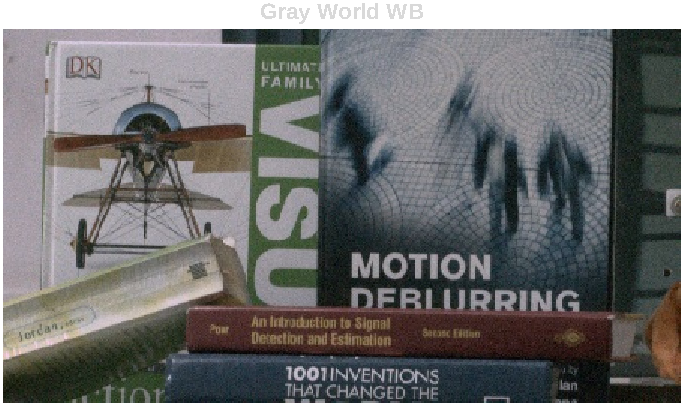
\includegraphics[width=\linewidth]{../output/RawImage1_WB_2.pdf}
							\caption{Gray World WB}
							\label{fig:RawImage1_WB_2}
						\end{subfigure}\\
						\begin{subfigure}[h]{0.45\linewidth}
							\centering
							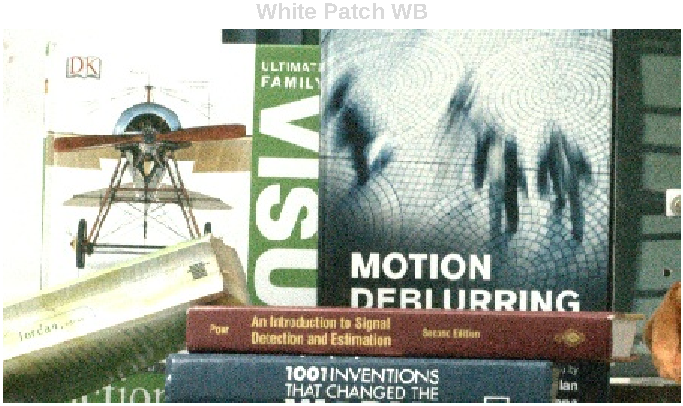
\includegraphics[width=\linewidth]{../output/RawImage1_WB_3.pdf}
							\caption{White Patch WB}
							\label{fig:RawImage1_WB_3}
						\end{subfigure} &
						\begin{subfigure}[h]{0.45\linewidth}
							\centering
							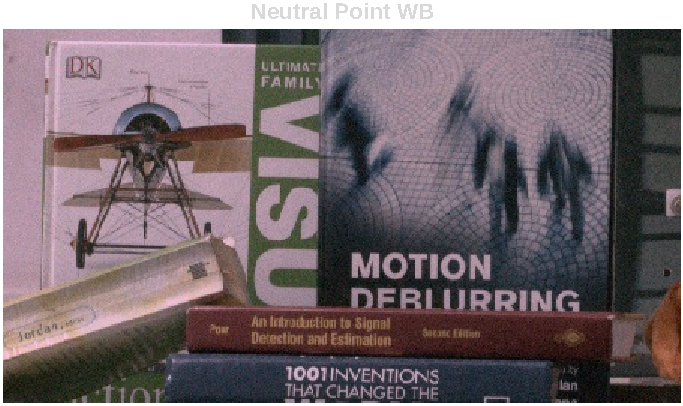
\includegraphics[width=\linewidth]{../output/RawImage1_WB_4.pdf}
							\caption{Neutral Point WB}
							\label{fig:RawImage1_WB_4}
						\end{subfigure}
					\end{tabular}
				}
				\caption{\texttt{RawImage1}-White Balance}
				\label{fig:RawImage1_WB}
			\end{figure}
			\begin{figure}[H]
				\centering
				\resizebox{0.8\linewidth}{!}{
					\begin{tabular}{cc}
						\begin{subfigure}[h]{0.45\linewidth}
							\centering
							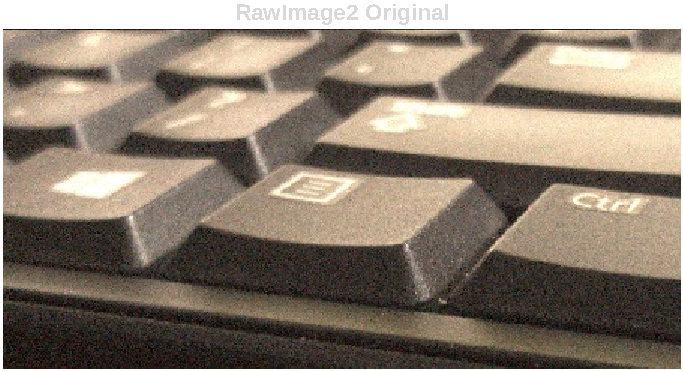
\includegraphics[width=\linewidth]{../output/RawImage2_WB_1.pdf}
							\caption{RawImage2 Original}
							\label{fig:RawImage2_WB_1}
						\end{subfigure} &
						\begin{subfigure}[h]{0.45\linewidth}
							\centering
							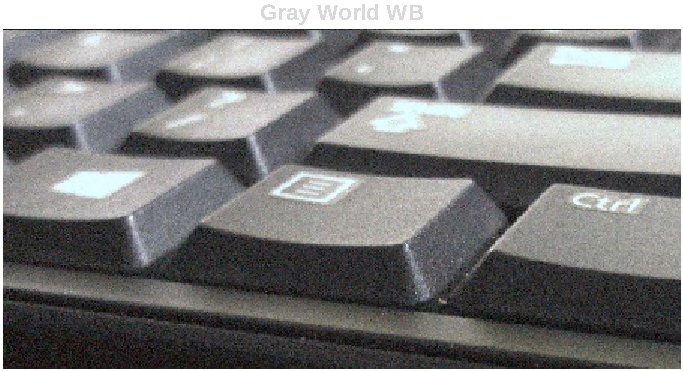
\includegraphics[width=\linewidth]{../output/RawImage2_WB_2.pdf}
							\caption{Gray World WB}
							\label{fig:RawImage2_WB_2}
						\end{subfigure}\\
						\begin{subfigure}[h]{0.45\linewidth}
							\centering
							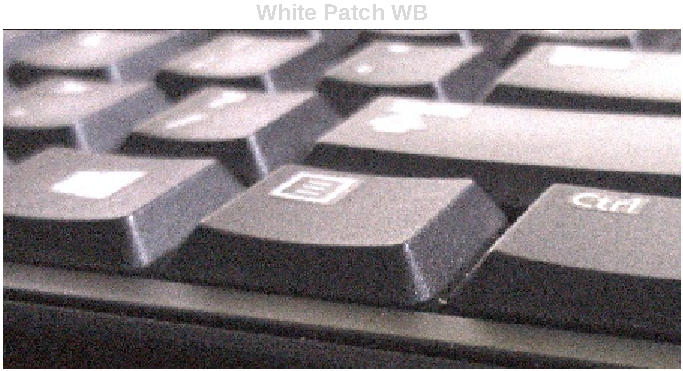
\includegraphics[width=\linewidth]{../output/RawImage2_WB_3.pdf}
							\caption{White Patch WB}
							\label{fig:RawImage2_WB_3}
						\end{subfigure} &
						\begin{subfigure}[h]{0.45\linewidth}
							\centering
							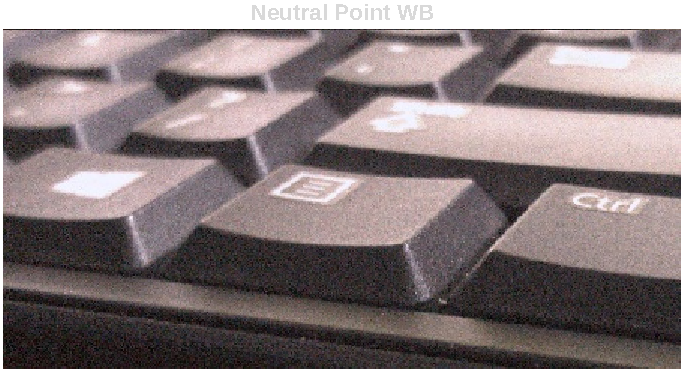
\includegraphics[width=\linewidth]{../output/RawImage2_WB_4.pdf}
							\caption{Neutral Point WB}
							\label{fig:RawImage2_WB_4}
						\end{subfigure}
					\end{tabular}
				}
				\caption{\texttt{RawImage2}-White Balance}
				\label{fig:RawImage2_WB}
			\end{figure}   
			\begin{figure}[H]
				\centering
				\resizebox{0.8\linewidth}{!}{
					\begin{tabular}{cc}
						\begin{subfigure}[h]{0.45\linewidth}
							\centering
							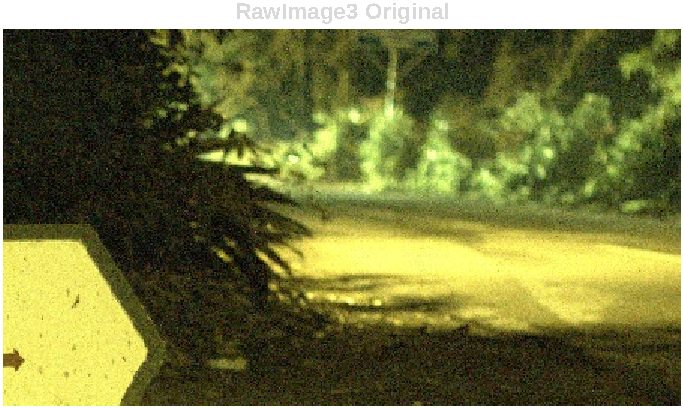
\includegraphics[width=\linewidth]{../output/RawImage3_WB_1.pdf}
							\caption{RawImage3 Original}
							\label{fig:RawImage3_WB_1}
						\end{subfigure} &
						\begin{subfigure}[h]{0.45\linewidth}
							\centering
							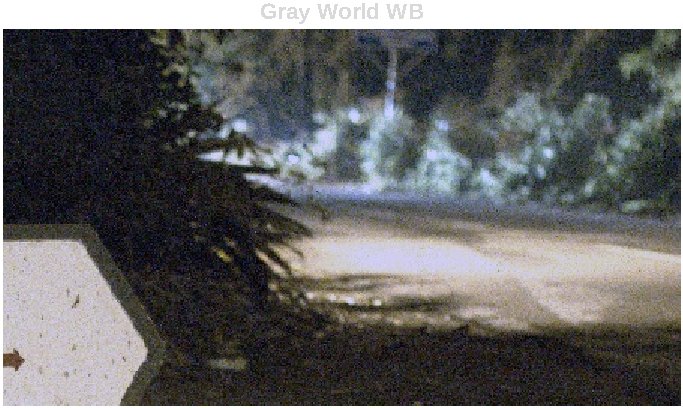
\includegraphics[width=\linewidth]{../output/RawImage3_WB_2.pdf}
							\caption{Gray World WB}
							\label{fig:RawImage3_WB_2}
						\end{subfigure}\\
						\begin{subfigure}[h]{0.45\linewidth}
							\centering
							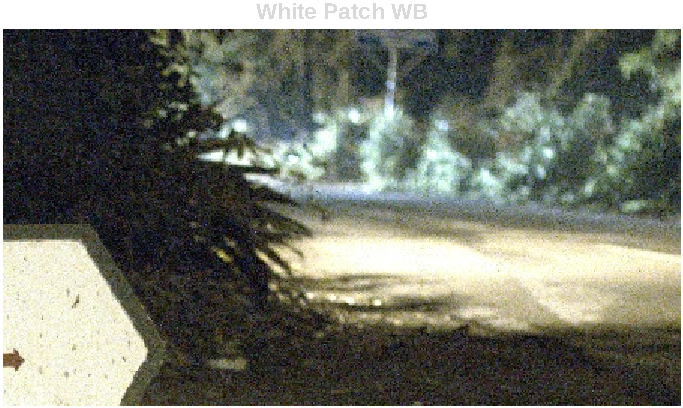
\includegraphics[width=\linewidth]{../output/RawImage3_WB_3.pdf}
							\caption{White Patch WB}
							\label{fig:RawImage3_WB_3}
						\end{subfigure} &
						\begin{subfigure}[h]{0.45\linewidth}
							\centering
							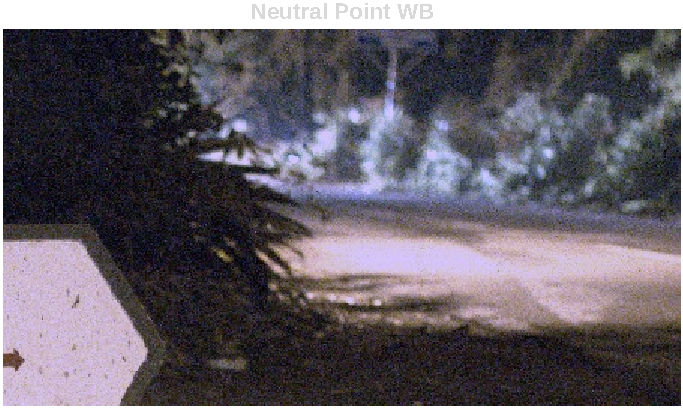
\includegraphics[width=\linewidth]{../output/RawImage3_WB_4.pdf}
							\caption{Neutral Point WB}
							\label{fig:RawImage3_WB_4}
						\end{subfigure}
					\end{tabular}
				}
				\caption{\texttt{RawImage3}-White Balance}
				\label{fig:RawImage3_WB}
			\end{figure}
			\begin{figure}[h]
				\centering
				\resizebox{\linewidth}{!}{
					\begin{tabular}{cccc}
						\begin{subfigure}[h]{0.45\linewidth}
							\centering
							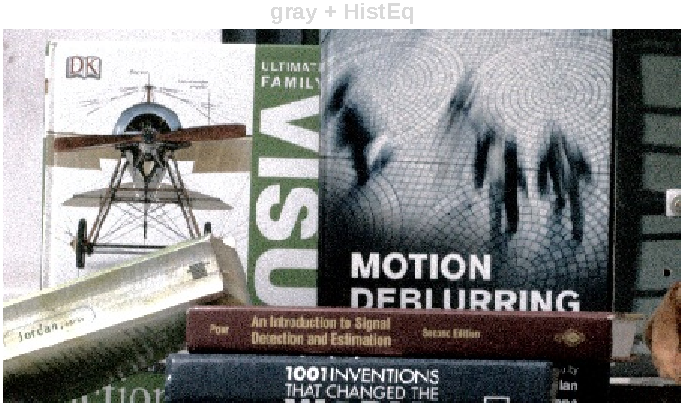
\includegraphics[width=\linewidth]{../output/RawImage1_Tone_gray_HistEq.pdf}
							\caption{gray+HistEq}
							\label{fig:RawImage1_tone_1}
						\end{subfigure} &
						\begin{subfigure}[h]{0.45\linewidth}
							\centering
							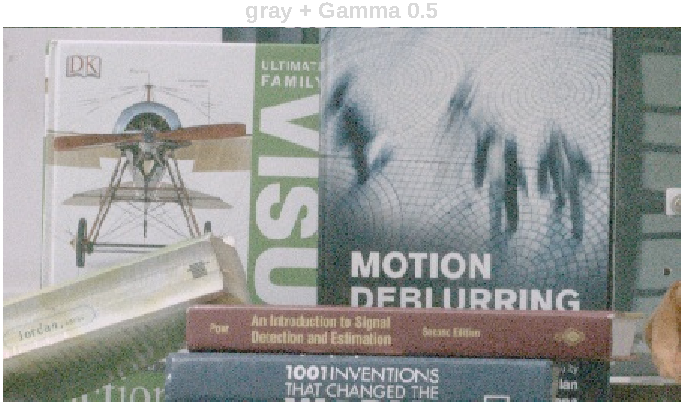
\includegraphics[width=\linewidth]{../output/RawImage1_Tone_gray_Gamma0.5.pdf}
							\caption{gray+Gamma 0.5}
							\label{fig:RawImage1_tone_2}
						\end{subfigure} &
						\begin{subfigure}[h]{0.45\linewidth}
							\centering
							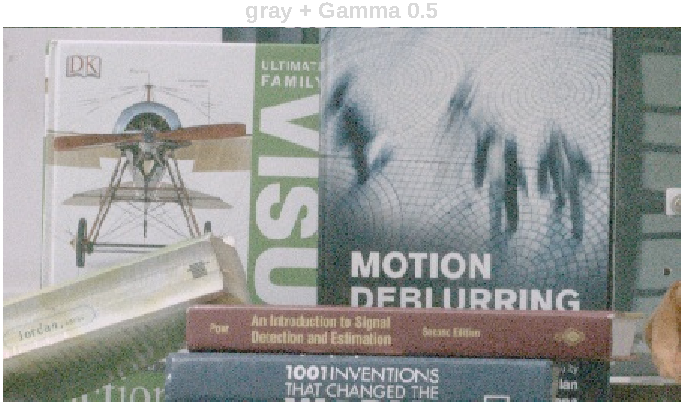
\includegraphics[width=\linewidth]{../output/RawImage1_Tone_gray_Gamma0.5.pdf}
							\caption{gray+Gamma 0.7}
							\label{fig:RawImage1_tone_3}
						\end{subfigure} &
						\begin{subfigure}[h]{0.45\linewidth}
							\centering
							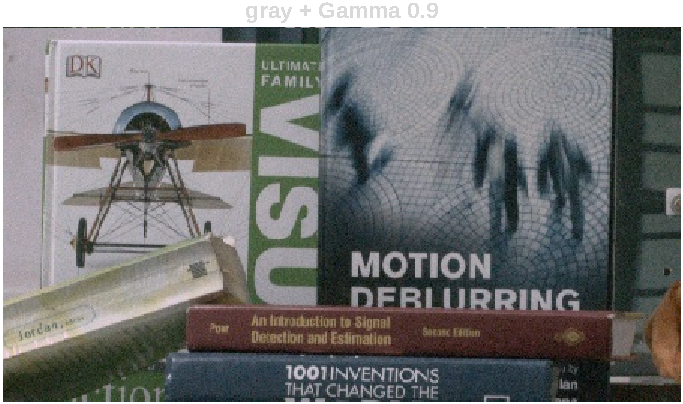
\includegraphics[width=\linewidth]{../output/RawImage1_Tone_gray_Gamma0.9.pdf}
							\caption{gray+Gamma 0.9}
							\label{fig:RawImage1_tone_4}
						\end{subfigure}\\
						\begin{subfigure}[h]{0.45\linewidth}
							\centering
							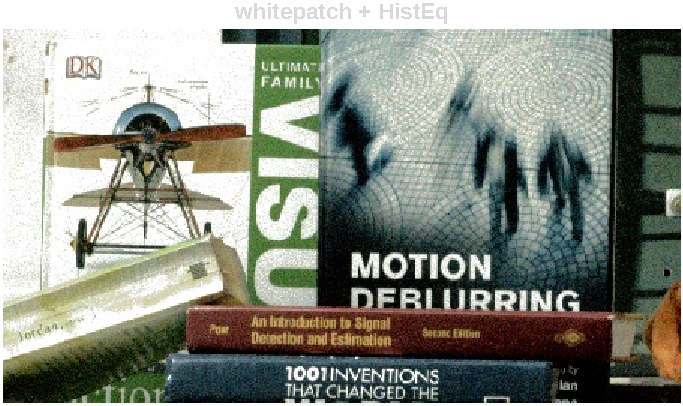
\includegraphics[width=\linewidth]{../output/RawImage1_Tone_whitepatch_HistEq.pdf}
							\caption{whitepatch+HistEq}
							\label{fig:RawImage1_tone_5}
						\end{subfigure} &
						\begin{subfigure}[h]{0.45\linewidth}
							\centering
							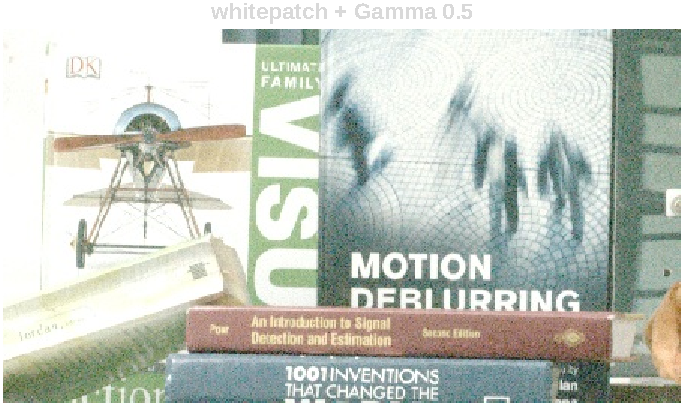
\includegraphics[width=\linewidth]{../output/RawImage1_Tone_whitepatch_Gamma0.5.pdf}
							\caption{whitepatch+Gamma 0.5}
							\label{fig:RawImage1_tone_6}
						\end{subfigure} &
						\begin{subfigure}[h]{0.45\linewidth}
							\centering
							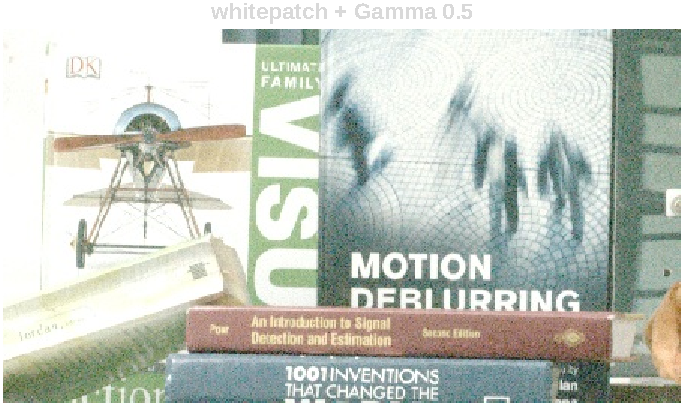
\includegraphics[width=\linewidth]{../output/RawImage1_Tone_whitepatch_Gamma0.5.pdf}
							\caption{whitepatch+Gamma 0.7}
							\label{fig:RawImage1_tone_7}
						\end{subfigure} &
						\begin{subfigure}[h]{0.45\linewidth}
							\centering
							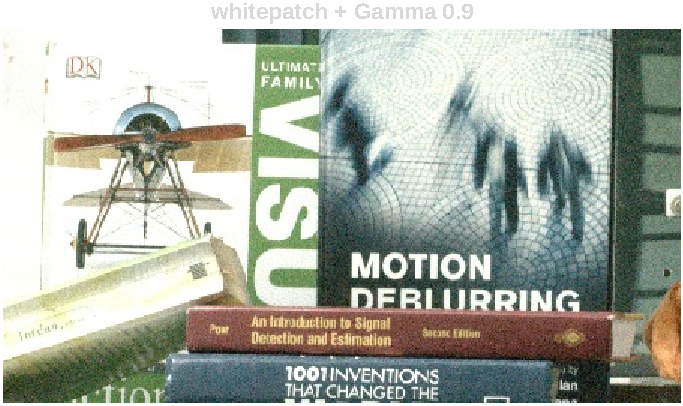
\includegraphics[width=\linewidth]{../output/RawImage1_Tone_whitepatch_Gamma0.9.pdf}
							\caption{whitepatch+Gamma 0.9}
							\label{fig:RawImage1_tone_8}
						\end{subfigure}\\
						\begin{subfigure}[h]{0.45\linewidth}
							\centering
							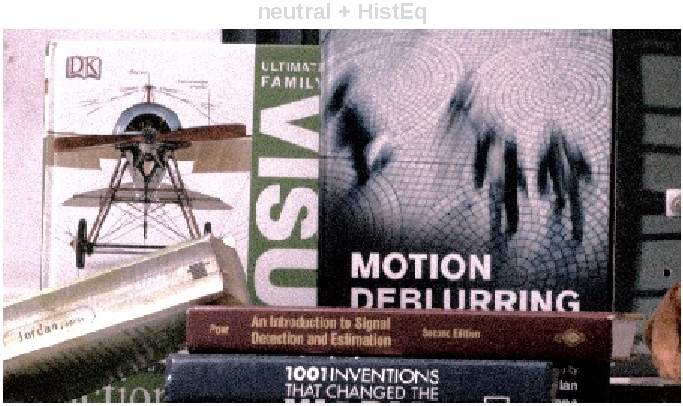
\includegraphics[width=\linewidth]{../output/RawImage1_Tone_neutral_HistEq.pdf}
							\caption{neutral+HistEq}
							\label{fig:RawImage1_tone_9}
						\end{subfigure} &
						\begin{subfigure}[h]{0.45\linewidth}
							\centering
							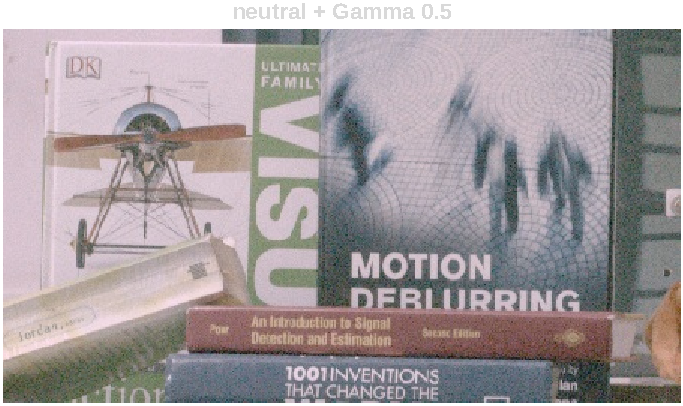
\includegraphics[width=\linewidth]{../output/RawImage1_Tone_neutral_Gamma0.5.pdf}
							\caption{neutral+Gamma 0.5}
							\label{fig:RawImage1_tone_10}
						\end{subfigure} &
						\begin{subfigure}[h]{0.45\linewidth}
							\centering
							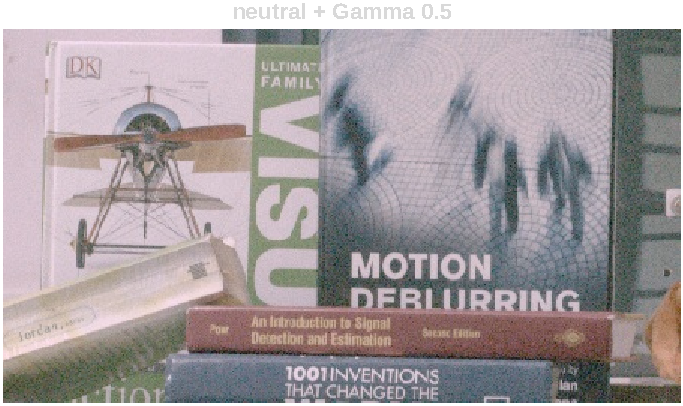
\includegraphics[width=\linewidth]{../output/RawImage1_Tone_neutral_Gamma0.5.pdf}
							\caption{neutral+Gamma 0.7}
							\label{fig:RawImage1_tone_11}
						\end{subfigure} &
						\begin{subfigure}[h]{0.45\linewidth}
							\centering
							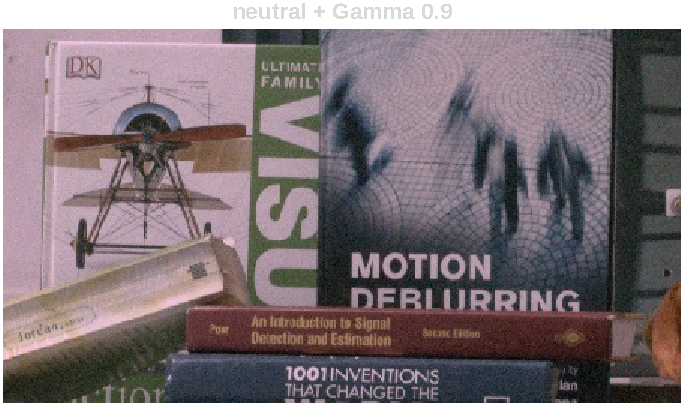
\includegraphics[width=\linewidth]{../output/RawImage1_Tone_neutral_Gamma0.9.pdf}
							\caption{neutral+Gamma 0.9}
							\label{fig:RawImage1_tone_12}
						\end{subfigure}
					\end{tabular}
				}
				\caption{\texttt{RawImage1}-tone mapping}
				\label{fig:RawImage1_tone}
			\end{figure}
			\begin{figure}[H]
				\centering
				\resizebox{\linewidth}{!}{
					\begin{tabular}{cccc}
						\begin{subfigure}[h]{0.45\linewidth}
							\centering
							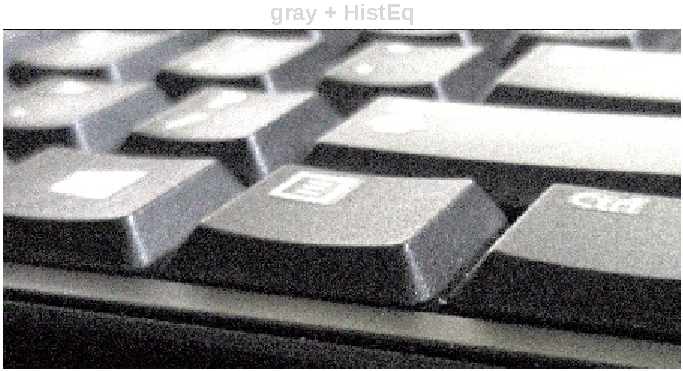
\includegraphics[width=\linewidth]{../output/RawImage2_Tone_gray_HistEq.pdf}
							\caption{gray+HistEq}
							\label{fig:RawImage2_tone_1}
						\end{subfigure} &
						\begin{subfigure}[h]{0.45\linewidth}
							\centering
							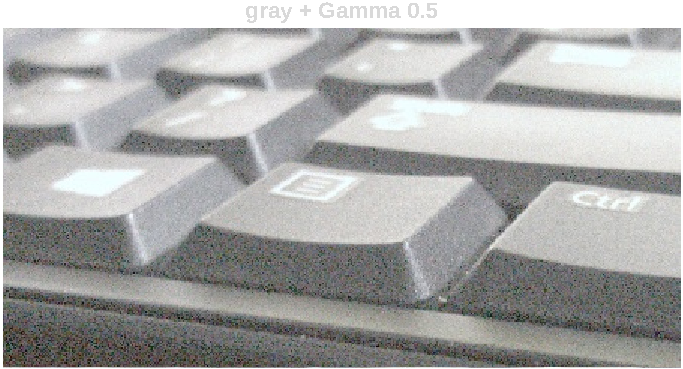
\includegraphics[width=\linewidth]{../output/RawImage2_Tone_gray_Gamma0.5.pdf}
							\caption{gray+Gamma 0.5}
							\label{fig:RawImage2_tone_2}
						\end{subfigure} &
						\begin{subfigure}[h]{0.45\linewidth}
							\centering
							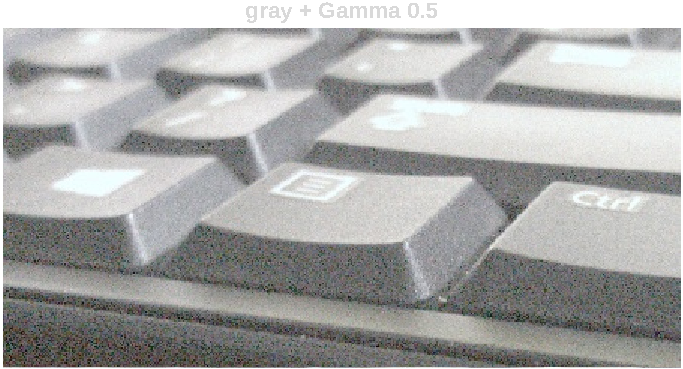
\includegraphics[width=\linewidth]{../output/RawImage2_Tone_gray_Gamma0.5.pdf}
							\caption{gray+Gamma 0.7}
							\label{fig:RawImage2_tone_3}
						\end{subfigure} &
						\begin{subfigure}[h]{0.45\linewidth}
							\centering
							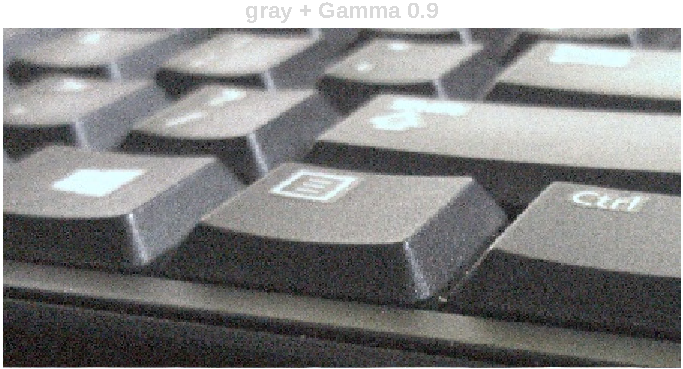
\includegraphics[width=\linewidth]{../output/RawImage2_Tone_gray_Gamma0.9.pdf}
							\caption{gray+Gamma 0.9}
							\label{fig:RawImage2_tone_4}
						\end{subfigure}\\
						\begin{subfigure}[h]{0.45\linewidth}
							\centering
							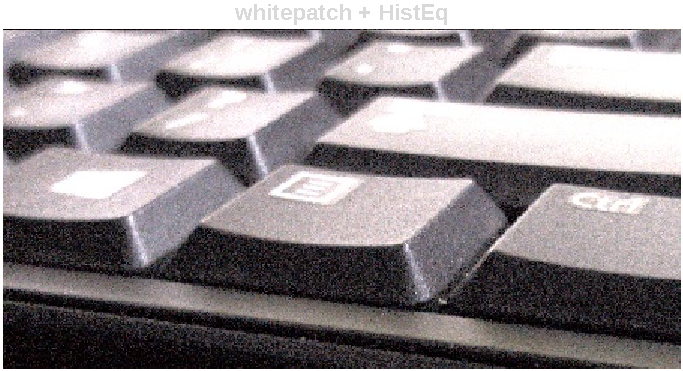
\includegraphics[width=\linewidth]{../output/RawImage2_Tone_whitepatch_HistEq.pdf}
							\caption{whitepatch+HistEq}
							\label{fig:RawImage2_tone_5}
						\end{subfigure} &
						\begin{subfigure}[h]{0.45\linewidth}
							\centering
							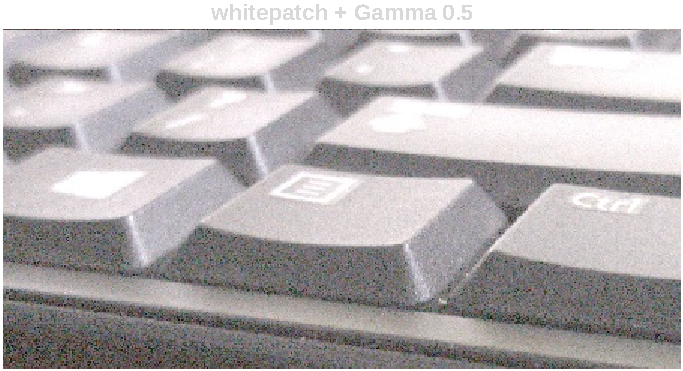
\includegraphics[width=\linewidth]{../output/RawImage2_Tone_whitepatch_Gamma0.5.pdf}
							\caption{whitepatch+Gamma 0.5}
							\label{fig:RawImage2_tone_6}
						\end{subfigure} &
						\begin{subfigure}[h]{0.45\linewidth}
							\centering
							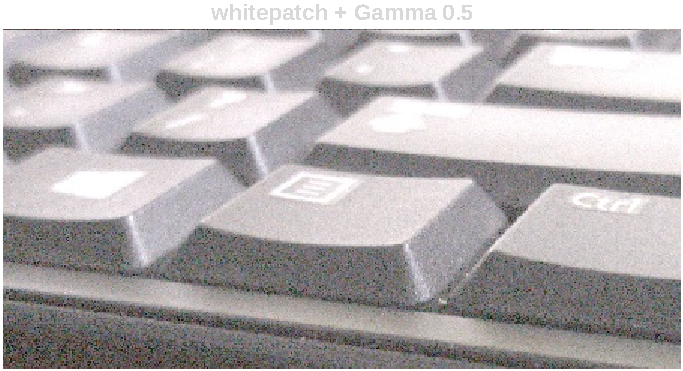
\includegraphics[width=\linewidth]{../output/RawImage2_Tone_whitepatch_Gamma0.5.pdf}
							\caption{whitepatch+Gamma 0.7}
							\label{fig:RawImage2_tone_7}
						\end{subfigure} &
						\begin{subfigure}[h]{0.45\linewidth}
							\centering
							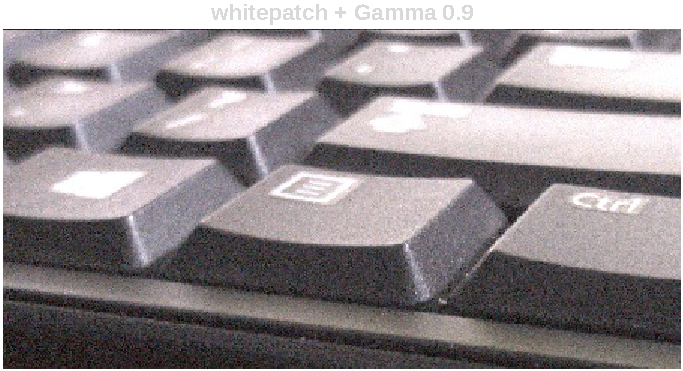
\includegraphics[width=\linewidth]{../output/RawImage2_Tone_whitepatch_Gamma0.9.pdf}
							\caption{whitepatch+Gamma 0.9}
							\label{fig:RawImage2_tone_8}
						\end{subfigure}\\
						\begin{subfigure}[h]{0.45\linewidth}
							\centering
							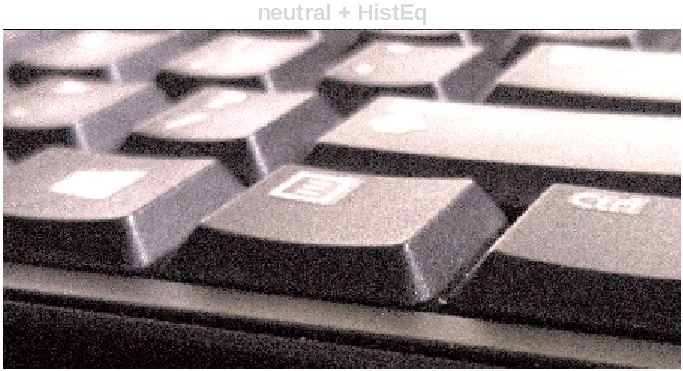
\includegraphics[width=\linewidth]{../output/RawImage2_Tone_neutral_HistEq.pdf}
							\caption{neutral+HistEq}
							\label{fig:RawImage2_tone_9}
						\end{subfigure} &
						\begin{subfigure}[h]{0.45\linewidth}
							\centering
							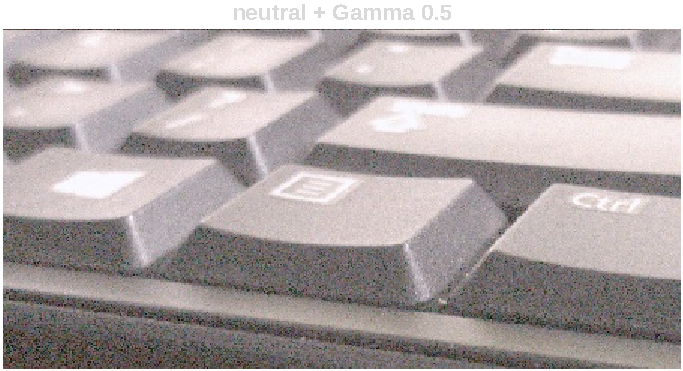
\includegraphics[width=\linewidth]{../output/RawImage2_Tone_neutral_Gamma0.5.pdf}
							\caption{neutral+Gamma 0.5}
							\label{fig:RawImage2_tone_10}
						\end{subfigure} &
						\begin{subfigure}[h]{0.45\linewidth}
							\centering
							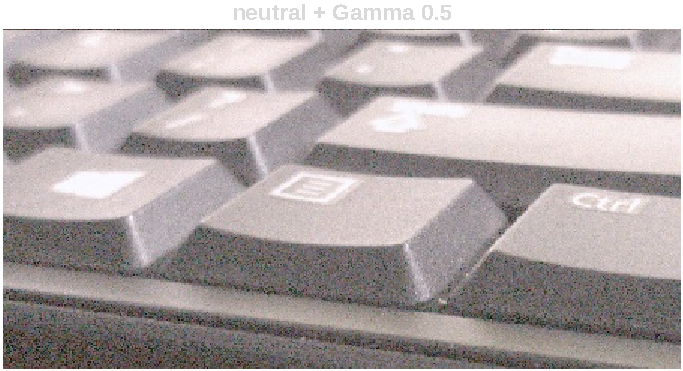
\includegraphics[width=\linewidth]{../output/RawImage2_Tone_neutral_Gamma0.5.pdf}
							\caption{neutral+Gamma 0.7}
							\label{fig:RawImage2_tone_11}
						\end{subfigure} &
						\begin{subfigure}[h]{0.45\linewidth}
							\centering
							\includegraphics[width=\linewidth]{../output/RawImage2_Tone_neutral_Gamma0.9.pdf}
							\caption{neutral+Gamma 0.9}
							\label{fig:RawImage2_tone_12}
						\end{subfigure}
					\end{tabular}
				}
				\caption{\texttt{RawImage2}-tone mapping}
				\label{fig:RawImage2_tone}
			\end{figure}
			\begin{figure}[H]
				\centering
				\resizebox{\linewidth}{!}{
					\begin{tabular}{cccc}
						\begin{subfigure}[h]{0.45\linewidth}
							\centering
							\includegraphics[width=\linewidth]{../output/RawImage3_Tone_gray_HistEq.pdf}
							\caption{gray+HistEq}
							\label{fig:RawImage3_tone_1}
						\end{subfigure} &
						\begin{subfigure}[h]{0.45\linewidth}
							\centering
							\includegraphics[width=\linewidth]{../output/RawImage3_Tone_gray_Gamma0.5.pdf}
							\caption{gray+Gamma 0.5}
							\label{fig:RawImage3_tone_2}
						\end{subfigure} &
						\begin{subfigure}[h]{0.45\linewidth}
							\centering
							\includegraphics[width=\linewidth]{../output/RawImage3_Tone_gray_Gamma0.5.pdf}
							\caption{gray+Gamma 0.7}
							\label{fig:RawImage3_tone_3}
						\end{subfigure} &
						\begin{subfigure}[h]{0.45\linewidth}
							\centering
							\includegraphics[width=\linewidth]{../output/RawImage3_Tone_gray_Gamma0.9.pdf}
							\caption{gray+Gamma 0.9}
							\label{fig:RawImage3_tone_4}
						\end{subfigure}\\
						\begin{subfigure}[h]{0.45\linewidth}
							\centering
							\includegraphics[width=\linewidth]{../output/RawImage3_Tone_whitepatch_HistEq.pdf}
							\caption{whitepatch+HistEq}
							\label{fig:RawImage3_tone_5}
						\end{subfigure} &
						\begin{subfigure}[h]{0.45\linewidth}
							\centering
							\includegraphics[width=\linewidth]{../output/RawImage3_Tone_whitepatch_Gamma0.5.pdf}
							\caption{whitepatch+Gamma 0.5}
							\label{fig:RawImage3_tone_6}
						\end{subfigure} &
						\begin{subfigure}[h]{0.45\linewidth}
							\centering
							\includegraphics[width=\linewidth]{../output/RawImage3_Tone_whitepatch_Gamma0.5.pdf}
							\caption{whitepatch+Gamma 0.7}
							\label{fig:RawImage3_tone_7}
						\end{subfigure} &
						\begin{subfigure}[h]{0.45\linewidth}
							\centering
							\includegraphics[width=\linewidth]{../output/RawImage3_Tone_whitepatch_Gamma0.9.pdf}
							\caption{whitepatch+Gamma 0.9}
							\label{fig:RawImage3_tone_8}
						\end{subfigure}\\
						\begin{subfigure}[h]{0.45\linewidth}
							\centering
							\includegraphics[width=\linewidth]{../output/RawImage3_Tone_neutral_HistEq.pdf}
							\caption{neutral+HistEq}
							\label{fig:RawImage3_tone_9}
						\end{subfigure} &
						\begin{subfigure}[h]{0.45\linewidth}
							\centering
							\includegraphics[width=\linewidth]{../output/RawImage3_Tone_neutral_Gamma0.5.pdf}
							\caption{neutral+Gamma 0.5}
							\label{fig:RawImage3_tone_10}
						\end{subfigure} &
						\begin{subfigure}[h]{0.45\linewidth}
							\centering
							\includegraphics[width=\linewidth]{../output/RawImage3_Tone_neutral_Gamma0.5.pdf}
							\caption{neutral+Gamma 0.7}
							\label{fig:RawImage3_tone_11}
						\end{subfigure} &
						\begin{subfigure}[h]{0.45\linewidth}
							\centering
							\includegraphics[width=\linewidth]{../output/RawImage3_Tone_neutral_Gamma0.9.pdf}
							\caption{neutral+Gamma 0.9}
							\label{fig:RawImage3_tone_12}
						\end{subfigure}
					\end{tabular}
				}
				\caption{\texttt{RawImage3}-tone mapping}
				\label{fig:RawImage3_tone}
			\end{figure}
		\item \textbf{Image Denoising}\\
		In this section, we employ bilateral filtering for image denoising. The bilateral filter is governed by two parameters, $\sigma_s$ and $\sigma_r$, which control the spatial weighting and the intensity alignment, respectively.  
		Ideally, one would locally estimate the noise level and adapt these parameters accordingly; however, due to computational cost, we use a fixed set of parameters.  
		
		To estimate the noise, a constant region is selected from each image, and the standard deviation is computed across the three channels (R, G, and B) within that region. The chosen filter parameters are:  
		\[
		W = 11, \quad \sigma_s = 2.5, \quad \sigma_r = 1.95 \times \sigma_n,
		\]
		where $\sigma_n$ denotes the noise standard deviation for the corresponding color channel.  
		
		The selected regions are:  
		\begin{enumerate}
			\item \texttt{RawImage1}: $(100, 100) \text{ to } (160, 160)$
			\item \texttt{RawImage2}: $(705, 924) \text{ to } (765, 984)$
			\item \texttt{RawImage3}: $(50, 400) \text{ to } (110, 460)$
		\end{enumerate}
		
		These regions are shown with red box in Figures~\ref{fig:RawImage1_denoising_1}, \ref{fig:RawImage2_denoising_1}, and \ref{fig:RawImage3_denoising_1}, corresponding to \texttt{RawImage1}, \texttt{RawImage2}, and \texttt{RawImage3}, respectively.  
		
		The estimated values of $\sigma_r$ for the R, G, and B channels are as follows:  
		\begin{itemize}
			\item \texttt{RawImage1}: $0.068$, $0.0614$, $0.0774$
			\item \texttt{RawImage2}: $0.0682$, $0.0510$, $0.0729$
			\item \texttt{RawImage3}: $0.0694$, $0.0694$, $0.1202$
		\end{itemize}
		
		The denoised results for \texttt{RawImage1}, \texttt{RawImage2}, and \texttt{RawImage3} are shown in Figures~\ref{fig:RawImage1_denoising_2}, \ref{fig:RawImage2_denoising_2}, and \ref{fig:RawImage3_denoising_2}, respectively.
		
			\begin{figure}[H]
				\centering
				\resizebox{0.8\linewidth}{!}{
					\begin{tabular}{cc}
						\begin{subfigure}[h]{0.45\linewidth}
							\centering
							\includegraphics[width=\linewidth]{../output/RawImage1_before_denoising.pdf}
							\caption{\texttt{RawImage1}-before Denoising}
							\label{fig:RawImage1_denoising_1}
						\end{subfigure} &
						\begin{subfigure}[h]{0.45\linewidth}
							\centering
							\includegraphics[width=\linewidth]{../output/RawImage1_after_denoising.pdf}
							\caption{\texttt{RawImage1}-after Denoising}
							\label{fig:RawImage1_denoising_2}
						\end{subfigure}\\
						\begin{subfigure}[h]{0.45\linewidth}
							\centering
							\includegraphics[width=\linewidth]{../output/RawImage2_before_denoising.pdf}
							\caption{\texttt{RawImage2}-before Denoising}
							\label{fig:RawImage2_denoising_1}
						\end{subfigure} &
						\begin{subfigure}[h]{0.45\linewidth}
							\centering
							\includegraphics[width=\linewidth]{../output/RawImage2_after_denoising.pdf}
							\caption{\texttt{RawImage2}-after Denoising}
							\label{fig:RawImage2_denoising_2}
						\end{subfigure}\\
						\begin{subfigure}[h]{0.45\linewidth}
						\centering
						\includegraphics[width=\linewidth]{../output/RawImage3_before_denoising.pdf}
						\caption{\texttt{RawImage3}-before Denoising}
						\label{fig:RawImage3_denoising_1}
						\end{subfigure} &
						\begin{subfigure}[h]{0.45\linewidth}
						\centering
						\includegraphics[width=\linewidth]{../output/RawImage3_after_denoising.pdf}
						\caption{\texttt{RawImage3}-after Denoising}
						\label{fig:RawImage3_denoising_2}
						\end{subfigure}
					\end{tabular}
				}
				\caption{Denoising}
				\label{fig:RawImages_denosising}
			\end{figure}
			\item \textbf{Questions:}\\
			\begin{enumerate}[label=\arabic*., start=1]
				\item Since a Gaussian distribution has infinite support, we must truncate it when constructing a discrete approximation. This truncation must be done carefully. For a given standard deviation $\sigma$, the kernel size is selected as the smallest odd integer greater than or equal to $6\sigma$. This choice is justified because approximately $99\%$ of the Gaussian’s total mass lies within a radius of $3\sigma$ around the mean. Thus, by taking $6\sigma$ as the kernel size, we effectively capture the essential structure of the Gaussian. Moreover, choosing an odd-sized kernel ensures the presence of a well-defined central pixel, allowing the kernel to be symmetrically aligned with pixels in the input image.
				\item $\sigma_r$ acts as a soft threshold to distinguish genuine edge differences from variations caused by noise. In practice, $\sigma_r$ should be chosen larger than $\sigma_n$, but not excessively so, since both extremes lead to undesirable effects.  
				
				\begin{itemize}
					\item \textbf{If $\boldsymbol{\sigma_r \leq \sigma_n}$:}  
					Even pixels with slightly different intensities from the reference pixel receive very low weights. Such small variations often arise purely from noise, particularly in flat regions. As a result, neighboring pixels do not contribute effectively to denoising, and little to no noise reduction is achieved.  
					
					\item \textbf{If $\boldsymbol{\sigma_r \gg \sigma_n}$:}  
					Pixels with large intensity differences still receive considerable weights, causing excessive averaging. This oversmoothing effect blurs edges and reduces important structural details in the image.  
				\end{itemize}
				
				These effects were verified experimentally using $\sigma_r = 0.95\sigma_n$ and $\sigma_r = 95\sigma_n$.  
				Based on these observations, a good practical choice is $\sigma_r \approx 2\sigma_n$.  
				
			\end{enumerate}
		\end{enumerate}
\end{document}